\documentclass{report}
\usepackage[utf8]{inputenc}
\usepackage{simpler-wick}
\usepackage{slashed}
\usepackage{appendix}
\usepackage{amsmath, amssymb}
\usepackage{tikz-feynman}
\usepackage{verbatim}

\title{An Analysis of the Scattering Matrix}
\author{Jack Hudson \\ Ridgefield High School \\ Advised by David Waltimyer}
\date{March 2021}

\begin{document}

\maketitle

\begin{abstract}
The goal of quantum physics is to describe the very smallest building blocks of our universe. One concept central to this describe is the idea of a scattering event, in which one particle collides with another, oftentimes at very high speeds. A useful tool when analyzing scattering events is the scattering matrix, or S-matrix, which relates the state of a system before a scattering event to the state of the system after the scattering event, thereby encoding all of the necessary information about the intermediate process.

In quantum mechanics, interactions between particles are described through potentials. In the first part of this discussion, the scattering matrix is introduced in the context of quantum mechanics. It is also computed for a number of trivial examples. However, it quickly becomes apparent that the tools of quantum mechanics are simply incapable of handling all but the simplest of scattering events. Thus is the motivation for a stronger theory: quantum field theory.

Initially, the benefits of quantum field theory are discussed. Following that, the Feynman path integral is introduced as well as the Feynman diagram, two pieces of machinery absolutely essential to the computation of scattering matrices in quantum field theory. Then, the Feynman rules are derived for scalar field theory, the simplest type of field theory, and the only one which shall be considered in this discussion. The first-order terms are computed for two interacting scalar field theories ($\Phi^4$ and $\Phi^3$), providing a template for computing matrix elements in more complex field theories.

After handling tree-level diagrams, the concept of renormalization is introduced, through which higher-order correction terms may be calculated. The process of Pauli-Villars regularization is described and implemented in order to compute the first higher-order correction to $\Phi^4$ theory, acting as an example which could be followed for other renormalizable theories.

Finally, the overall process for computing scattering matrix elements in any quantum field theory is explained, ending with a concise list of the steps which must be followed in the analysis of scattering.
\end{abstract}

\newpage
\tableofcontents

\newpage
\part{Quantum Mechanics}
\chapter{Scattering Experiments in Quantum Mechanics}
\section{What is Scattering?}
% Explain scattering experiments in general
At the heart of physics is the concept of an interaction: an event in which one thing has an effect on another in some way. Without interactions, physics would be, quite frankly, boring, with particles flying in straight lines, ignoring one another completely. Broadly, there are two types of interactions. The first is the type that leads to bound states--systems in which particles are "stuck" to one another. For instance, an electron and a proton can undergo a binding event, uniting them into perhaps the most well-known and heavily studied bound states: the hydrogen atom. On the other hand, the second type of interaction is known as a scattering event. It is this type of interaction which shall occupy us for the remainder of this endeavor.

Scattering events are interactions in which particles collide, interacting in some way as they do so. It turns out that each of the four fundamental forces--electromagnetism, gravity, and the strong and weak interactions--essentially operate through scattering. As with interactions, there are two types of scattering, so called "2 $\rightarrow n$" scattering and "1 $\rightarrow n$" scattering. The former consists of interactions in which two particles collide with one another and, through some intermediate process, particles fly out of the interaction. The resulting particles may be the same as the initial ones, for instance in the case of Møller scattering, when two electrons scatter off of one another and fly off in different directions. However, the resulting particles may be new. For example, when a muon collides with its antimatter counterpart, sometimes an electron-positron pair will come out, as if by magic.

1 $\rightarrow n$ scattering has a special name: decay. It is when a singular particle spontaneously becomes other, lighter particles in a more favorable configuration, for instance when a tauon spontaneously decays into two neutrinos and an electron. As nature would have it, only the weak interaction can mediate a decay. More complex scatterings, such as 3 $\rightarrow$ n or 4 $\rightarrow$ n are possible only in theory. Just you try smashing three subatomic particles into each other at exactly the same instant!

\section{Dirac Notation}
% Go over Dirac notation for a state, ending with the introduction of the scattering matrix as the time evolution operator
It is all well and good to understand what scattering is, but physics is useless without being able to make mathematical calculations which lead to physical predictions. In the early days of the development of quantum mechanics, Werner Heisenberg discovered that the theory could be very well descried using the language of linear algebra. In this sense, states are represented as column matrices, such that each basis vector is a basis state. As an example, let us consider an electron's spin. If $\begin{bmatrix} 1 \\ 0 \end{bmatrix}$ is defined as the spin-up state and $\begin{bmatrix} 0 \\ 1 \end{bmatrix}$ the spin-down state, then $\begin{bmatrix} \frac{1}{\sqrt{2}} \\ \frac{1}{\sqrt{2}} \end{bmatrix}$ is the electron's state if it is in perfectly equal superposition between spin-up and spin-down.

Following from this, the adjoint of a state (its complex conjugate transpose) is a row matrix. For the electron spin example, this is $\begin{bmatrix} \frac{1}{\sqrt{2}} & \frac{1}{\sqrt{2}} \end{bmatrix}$, because the state had no imaginary parts. Transformations are then operators, of (usually Hermitian) matrices. Continuing this example, the "flipping" transformation would be $\begin{bmatrix} 0 & 1 \\ 1 & 0 \end{bmatrix}$. Observables, as it turns out, are eigenvalues of certain operators, hence the incredibly succinct rendition of the Schrödinger equation: $\hat{H} \psi = E \psi$, where $\hat{H}$ is the Hamiltonian operator, $E$ is the energy, and $\psi$ is the column matrix representing the current state. As expected, the multiplication of a state by its adjoint produced either their inner or outer product, depending on the order of multiplication.

Paul Dirac invented a notation (aptly named Dirac Notation) for these ideas. States are represented as "ket vectors" $\vert \psi \rangle$, where $\psi$ is just the name of the state. For instance, $\vert \uparrow \rangle$ and $\vert \downarrow \rangle$ for the spin example. Adjoints are "bra vectors" $\langle \psi \vert$. Inner products between states are then $\langle a \vert b \rangle$, forming a "bra-ket", or "bracket", hence the name.

At this point, one may be wondering what all this has to do with scattering. Well, let us suppose we have some system with initial state $\vert i \rangle$ and final state $\vert f \rangle$. When the system is between these two states, some scattering event takes place, which we would like to study. We should be able to multiply $\vert i \rangle$ by some operator to produce $\vert f \rangle$. If this were the case (spoiler alert: it is) then that operator would encode all of the relevant information about the intermediate process without needing any information about the initial state. Then, given an initial state, we could utilize this operator to produce the final state. In general, this is called the time evolution operator, but the scattering case is special. Mathematically, its role is:
\[
\vert f \rangle = \hat{S} \vert i \rangle
\]
and in the case of scattering, this operator, $\hat{S}$, is known as the scattering matrix\footnote{It is also often referred to as the "s-matrix", and both terms will be used interchangeably.}.

\section{The Scattering Matrix}
% Go over the generalized scattering experiment and the intuition behind the scattering matrix in quantum mechanics
Scattering experiments in quantum mechanics are relatively straightforward, and make a few assumptions that simplify things even further. Perhaps most importantly, quantum mechanical scattering events assume that the particles are the same before and after the interaction. They also assume that interactions are localized enough that they are negligible at all but teh closest distances. In terms of setup, things are considered from the reference frame of one particle, and only the effects on the other particle are considered, which are expressed as some potential energy function only nonzero near the origin.

Pictographically, the experiment is:
\[
% Some text QMscatteringone
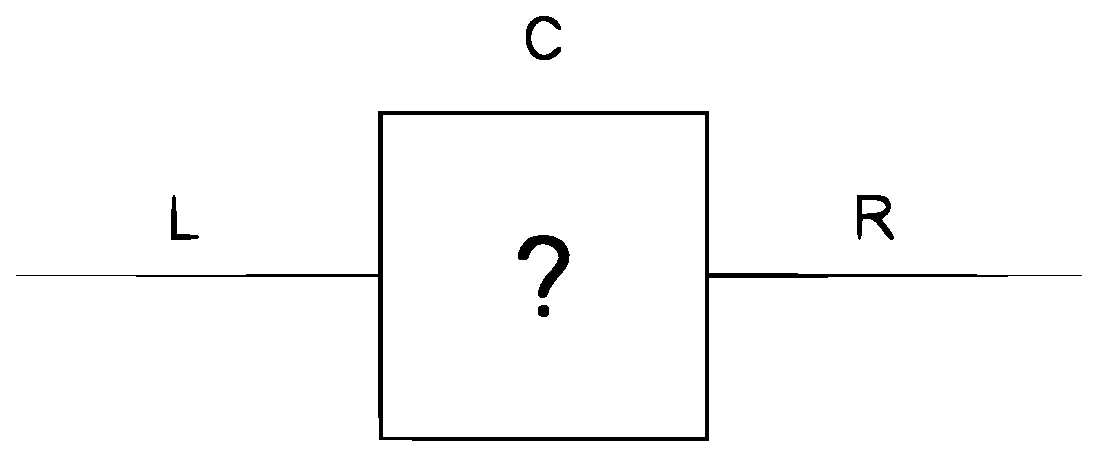
\includegraphics[scale=0.25]{QMscatteringone.eps}
\]
where the left (L), central (C), and right (R) regions are labelled.

The wavefunction of the particle in question can be broken up by region as well, into $\psi_L(x)$, $\psi_C(x)$, and $\psi_R(x)$. Each piecewise portion of the overall wavefunction must satisfy the Schrödinger equation in its domain\footnote{This is the time-independent Schrödinger equation, which we can use because the potential is not a function of time. Technically, the time dependent part of the wavefunction is $u(t) = e^{iEt}$, as per the time-dependent Schrödinger equation $E u(t) = -i \hbar \frac{\partial}{\partial t} u(t)$. Because the two parts were isolated via separation of variables, they combine to the proper wavefunction $\Psi (x, t) = \psi(x) u(t)$.}:
\[
\frac{-\hbar^2}{2m} \bigtriangledown^2 \psi(x) + V(x) \psi(x) = E \psi(x)
\]

In the left and right regions, the potential is 0, greatly simplifying the Schrödinger equation. Let us first consider only $\psi_L$.
\[
\frac{-\hbar^2}{2m} \frac{\partial^2}{{\partial x}^2} \psi_L(x) = E \psi_L(x)
\]
where we have also made the substitution $\bigtriangledown^2 = \frac{\partial^2}{{\partial x}^2}$, as this is a one-dimensional model. We can invent a variable $k = \frac{\sqrt{2mE}}{\hbar}$, yielding:
\[
\frac{\partial^2}{{\partial x}^2} \psi_L(x) = -k^2 E \psi_L(x)
\]

This is a very straightforward differential equation, with generalized solution:
\[
\psi_L(x) = Ae^{ikx} + Be^{-ikx}
\]
and by similar logic:
\[
\psi_R(x) = Ce^{ikx} + De^{-ikx}
\]

The first term of $\psi_L$ represents particles moving to the right, while the second term represents particles moving to the left, and likewise for $\psi_R$. Because the exponentials all have norm 1 (as $e^{i\theta}$ always has), $A$, $B$, $C$, and $D$ are the magnitudes of each of these terms. So:
\[
% Some text QMscatteringtwo
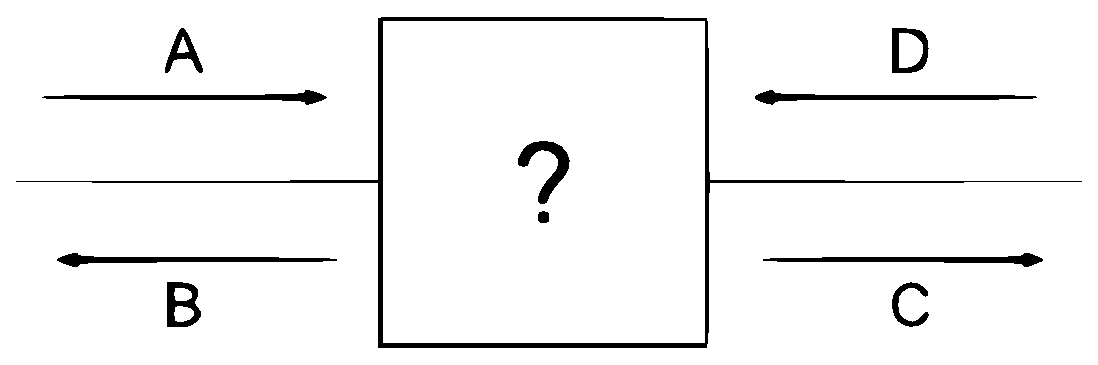
\includegraphics[scale=0.25]{QMscatteringtwo.eps}
\]

This means that $A$ and $D$ represent the incoming amplitudes, while $B$ and $C$ represent the outgoing amplitudes. This gives us a nice way to represent the initial and final states of our system, when the particle is either fully incoming or outgoing:
\[
\vert i \rangle = \begin{bmatrix} $A$ \\ $D$ \end{bmatrix}, \vert f \rangle = \begin{bmatrix} $B$ \\ $C$ \end{bmatrix}
\]

The scattering matrix is finally ready to make its appearance. By its very definition, the scattering matrix satisfies 
\[
\begin{bmatrix} $B$ \\ $C$ \end{bmatrix} =  \hat{S} \begin{bmatrix} $A$ \\ $D$ \end{bmatrix}
\]

Clearly, the scattering matrix must contain all of the information about the interaction itself, and so calculating it will satisfy out original goal: to study the interaction. However, the scattering matrix is different for each possible interaction, so we will need an example interaction before we can actually sit down and evaluate it.

\subsection{Transfer and Reflection Coefficients}
% Talk about the transfer and reflection coefficients, and why they are all that is needed to describe a realistic scattering matrix (because of mono-directional incoming beams)
Before we actually go about evaluating scattering matrices, there is one simplification we can make to ease the math. In the real world, scattering experiments rarely have an incoming particle in a superposition of entering from the right and the left. Realistically, the experiment will consist of some sort of monodirectional beam being shot at a potential. Therefore, we can ignore incoming particles from the right (equivalently, assume $\vert i \rangle = \begin{bmatrix} $A$ \\ $0$ \end{bmatrix}$) and calculate the left of of the scattering matrix, then ignore incoming particle from the right (assume $\vert i \rangle = \begin{bmatrix} $0$ \\ $D$ \end{bmatrix}$).

Let us consider for a moment the former situation--particles exclusively coming in from the left. In this case, we have $\hat{S}\begin{bmatrix} $A$ \\ $0$ \end{bmatrix} = \begin{bmatrix} $B$ \\ $C$ \end{bmatrix}$, so, by some simple matrix multiplication, $\hat{S}_{11} = \frac{B}{A}, \hat{S}_{21} = \frac{C}{A}$. Because no particles came in from the right, $\hat{S}_{11}$ is the magnitude of particles coming in from the left and leaving to the left. In other words, it represents the probability amplitude of a particle being reflected by the potential. Because we are not dealing with bound states, $\hat{S}_{21}$ represents the probability amplitude of particles being transmitted through the potential. For these reasons, $\hat{S}_{11}$ and $\hat{S}_{21}$ are called, respectively, the reflection coefficient $r$ and the transmission coefficient $t$.\footnote{Remember that this only applies when we only consider scattering from only one side.} These quantities' norms squared represent their respective probabilities, so the reflectivity $R = |r|^2$ and the transmissivity $T = |t|^2$.

\chapter{Simple Scattering Examples}
% Just calculate the scattering matrix for each of these examples 
\section{Free}
Oftentimes, the easiest test to perform to make sure your methods work is to try the free case. That is, the case in which there is no interaction, and particles simply move in straight lines. Whenever we develop a new theory or model, this will always be the first thing we try. Before we begin any calculations, let us consider what the scattering matrix should be for the free case.

For any symmetrical scattering potential (which the free case certainly is), the scattering matrix should be symmetric. This is because scattering coming in from the left will have the same probability amplitudes of reflecting and transmitting as scattering coming in from the right. This means that we need only calculate two elements of the scattering matrix (the two that come into play when we consider scattering coming only from the left), because we know that the other two (the two that come into play when we consider scattering coming only from the right) will be automatically found through the symmetry of the matrix.

As we found earlier, $S_{11}$ and $S_{21}$ should be the reflection and transmission coefficients, respectively, as this is a "scattering only from the left" calculation. In the free case, it does not take much thinking to conclude that the particle should only transmit through, as there is no interaction potential to reflect off of! So, because $R$ should be 0 and $T$ should be 1, $r$ will be 0, and $t$ will be some complex number with norm 1 (i.e. it will lie on the unit circle). This means that the scattering matrix should be $\begin{bmatrix} 0 & e^{i \theta} \\ e^{i \theta} & 0 \end{bmatrix}$, where $\theta$ is just some number parameterizing the options for $t$, which is fine because only its norm is an observable. Let us see if our intuition is correct!

The wavefunction to the left of the origin $\psi_L(x)$ is $Ae^{ikx} + Be^{-ikx}$ and to the right of the origin is $Ce^{ikx} + De^{-ikx}$. However, because we are only considering scattering from the left, $D=0$. Also, we are only interested in $r$ and $t$, not in $A$, $B$, or $C$. So, it would be nice if we could switch to speaking about the variables we are actually interested in. Fortunately, we can do this! First, recall that we are not normalizing these wavefunctions. This means that there is an implied constant scale factor being multiplied by the wavefunction, ensuring that the wavefunction is normalized\footnote{That is, that the integral of the wavefunction over all space is 1, or else there would be a chance other than 1 that the particle is "somewhere".}. This means that we can feel free to multiply our overall wavefunction by some constant without worrying about messing with the results, because it can be absorbed into the normalization constant. Multiplying by $\frac{1}{A}$ gives much nicer forms of the wavefunctions:
\[
\psi_L(x) = e^{ikx} + re^{ikx}, \psi_R(x) = te^{ikx}
\]

Now, as we have two unknowns ($r$ and $t$), we need two independent equations. These will both come from the rule of the continuity of the wavefunction: the wavefunction cannot have any discontinuities, nor can its derivative. Therefore, because our right and left wavefunctions "meet" at $x=0$, continuity requires:
\[
\psi_L(0) = \psi_R(0), \frac{\partial}{\partial x}\psi_L(0) = \frac{\partial}{\partial x}\psi_R(0)
\]

Inserting our expressions for the two halves of the wavefunction gives two very nice equations\footnote{The step of stating that $e^{ik(0)} = 1$ is implied.}:
\[
1 + r = t, 1 - r = t
\]
Combining these two equations gives
\[
1 - r = 1 + r
\]
To which the only solution is $r = 0$. Hooray, this is exactly what we anticipated! There is no reflection, and the particles freely propagate through space. Finishing up the calculation for posterity, $R = |r|^2 = 0$, implying $T = 1$, which, because $T = |t|^2$, has solution $t = e^{i\theta}$, where $\theta$ parameterizes the options for $t$. This gives the exact same matrix as before:
\[
\hat{S} = \begin{bmatrix} 0 & e^{i\theta} \\ e^{i\theta} & 0 \end{bmatrix}
\]

\section{Finite Barrier}
Unfortunately, the finite barrier problem is significantly more complex than the free case. The finite barrier potential consists of a region near the origin of length $l$ in which the potential is at a constant $V_0$. To simplify the mathematics, we shall consider the left boundary of the barrier to be at $x=0$ and the right boundary to be at $x = l$.

\[
% Some text finitebarrier
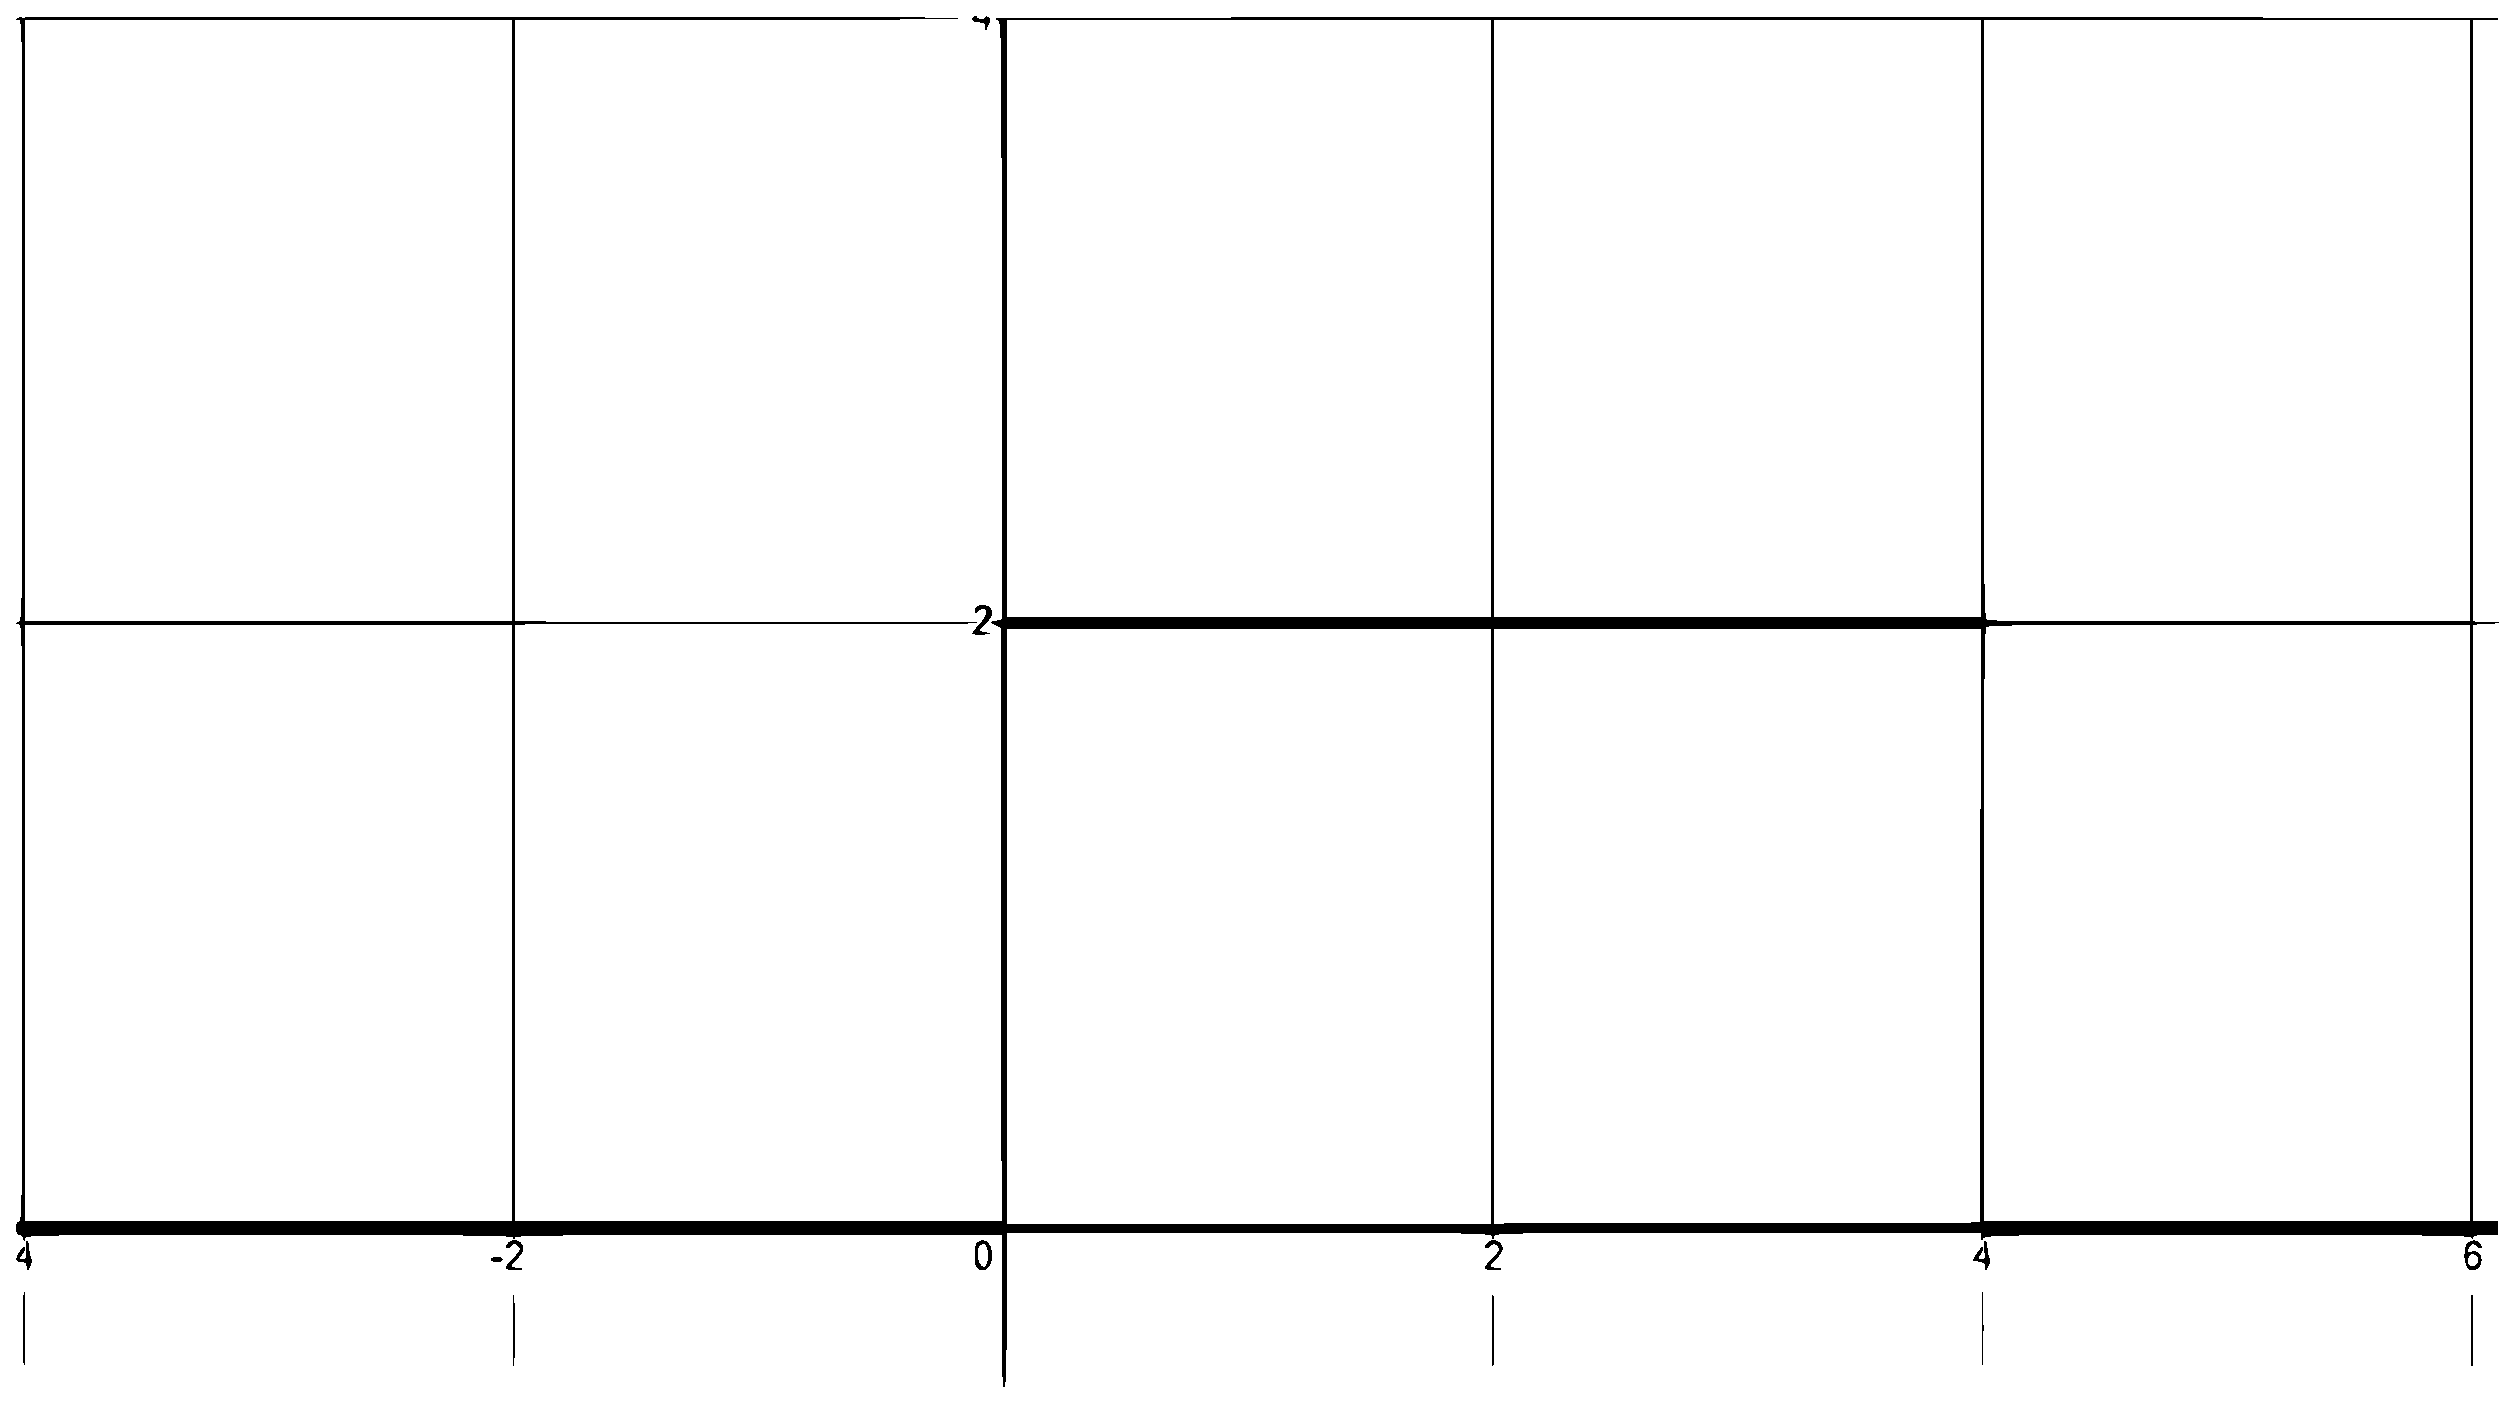
\includegraphics[scale=0.25]{finitebarrier.eps}
\]

Using the same trick as in the free case, we have the wavefunctions:
\[
\psi_L(x) = e^{ikx} + re^{ikx}, \psi_R(x) = te^{ikx}
\]
However, we need to find the central wavefunction. Using the Schrödinger equation:
\[
\frac{-\hbar^2}{2m} \frac{\partial^2}{{\partial x}^2} \psi_C(x) + V_0\psi_C(x) = E\psi_C(x)
\]
Rearranging,
\[
\frac{-\hbar^2}{2m} \frac{\partial^2}{{\partial x}^2} \psi_C(x) = (E-V_0)\psi_X(x)
\]
Or,
\[
\frac{\partial^2}{{\partial x}^2} \psi_C(x) = -\mathcal{K}^2\psi_X(x)
\]
where $\mathcal{K} = \frac{\sqrt{2m(E-V_0)}}{\hbar}$. This exactly the same differential equation as when the wavefunction is to the left or right of the potential, and so the general solution is of exactly the same form:
\[
\psi_C(x) = Fe^{i\mathcal{K}x} + Ge^{-i\mathcal{K}x}
\]

Now, we have twice as many variables as in the free case ($F$ and $G$ in addition to $r$ and $t$), but also two boundaries at which to ensure continuity. At the first boundary, continuity of the wavefunction and its derivative gives the two equations:
\[
1 + r = F + G, k(1 - r) = \mathcal{K}(F - G)
\]
Likewise, continuity at the second boundary gives:
\[
te^{ikl} = Fe^{i\mathcal{K}l} + Ge^{-i\mathcal{K}l}, kte^{ikl} = \mathcal{K}(Fe^{i\mathcal{K}l} - Ge^{-i\mathcal{K}l})
\]
To simplify things, let us define two new variables: $p = Fe^{i\mathcal{K}l}$ and $q = Ge^{-i\mathcal{K}l}$. Using these variables, the second boundary continuity equations become
\[
te^{ikl} = p + q, kte^{ikl} = \mathcal{K}(p - q)
\]
So, combining these two equations:
\[
\frac{\mathcal{K}}{k}(p - q) = p + q
\]
\[
\frac{\mathcal{K}}{k}p - \frac{\mathcal{K}}{k}q = p + q
\]
\[
(\frac{\mathcal{K}}{k} - 1)p = (\frac{\mathcal{K}}{k} + 1)q
\]
\[
p = \frac{\frac{\mathcal{K}}{k} + 1}{\frac{\mathcal{K}}{k} - 1}q
\]
Inserting this back into the earlier equation gives
\[
F = \frac{\frac{\mathcal{K}}{k} + 1}{\frac{\mathcal{K}}{k} - 1}e^{-2i\mathcal{K}l}G
\]
This is very cumbersome, so let us define a new constant $\xi = \frac{\frac{\mathcal{K}}{k} + 1}{\frac{\mathcal{K}}{k} - 1}e^{-2i\mathcal{K}l}$, so $F = \xi G$. Combining this with the first of the first boundary continuity equations gives
\[
1 + r = (\xi + 1)G
\]
so $G = \frac{1+r}{1+\xi}$. Inserting all of these identities into the second continuity equation for the first boundary will finally give us an equation of only $r$:
\[
k(1 - r) = \mathcal{K}(\frac{1+r}{1+\xi}\xi - \frac{1+r}{1+\xi}) = \frac{\mathcal{K}(1+r)}{1+\xi}(\xi - 1)
\]
Performing a slew of algebra to solve for $r$ gives our final result:
\[
r = \frac{k - \mathcal{K}\frac{\xi - 1}{\xi + 1}}{k + \mathcal{K}\frac{\xi - 1}{\xi + 1}}
\]
This gives the (monstrous) final scattering matrix:
\[
\hat{S} = \begin{bmatrix} \frac{k - \mathcal{K}\frac{\xi - 1}{\xi + 1}}{k + \mathcal{K}\frac{\xi - 1}{\xi + 1}} & \sqrt{1 - (\frac{k - \mathcal{K}\frac{\xi - 1}{\xi + 1}}{k + \mathcal{K}\frac{\xi - 1}{\xi + 1}})^2} \\ \sqrt{1 - (\frac{k - \mathcal{K}\frac{\xi - 1}{\xi + 1}}{k + \mathcal{K}\frac{\xi - 1}{\xi + 1}})^2} & \frac{k - \mathcal{K}\frac{\xi - 1}{\xi + 1}}{k + \mathcal{K}\frac{\xi - 1}{\xi + 1}} \end{bmatrix}
\]
Because of the matrix's complexity, is it far easier to deal with $r$ and $t$ alone, then generate the scattering matrix once they have already been found.

\subsection{Confirming the Free Theory}
To ensure that we have not made a significant mistake, let us now take a moment to confirm that this formula behaves as we would expect it to in the free theory. In the free theory, $\mathcal{K}$ goes to $k$. This means that:
\[
\xi = \lim_{\mathcal{K} \to k} \frac{\frac{\mathcal{K}}{k} + 1}{\frac{\mathcal{K}}{k} - 1}e^{-2i\mathcal{K}l}
\]
This blows up to infinity as $\mathcal{K}$ approaches $k$, and the denominator approaches 0. $r$ is given by $\frac{k - \mathcal{K}\frac{\xi - 1}{\xi + 1}}{k + \mathcal{K}\frac{\xi - 1}{\xi + 1}}$. Taking the limit,
\[
r = \lim_{\xi \to \infty, \mathcal{K} \to k} \frac{k - \mathcal{K}\frac{\xi - 1}{\xi + 1}}{k + \mathcal{K}\frac{\xi - 1}{\xi + 1}} = \lim_{\mathcal{K} \to k} \frac{k - \mathcal{K}}{k + \mathcal{K}} = 0
\]
So $r=0$, exactly as we would hope, giving the free scattering matrix as before.

\section{Quantum Tunneling}
% Just go straight into the example, and reveal why tunneling is contrary to classical intuition
There is something peculiar about our result for the finite barrier that will lead us to a fundamental and fascinating property of quantum mechanics. Let us consider a specific example of the finite barrier, where the length of the barrier $l$, the mass of our particle $m$, and the energy of the particle $E$ are all 1 in their respective units, for computational simplicity. The height of the potential barrier, though, will be taken to be 2 units. We will also be using natural units\footnote{c = $\hbar$ = 1}. As with the free case, let us use our intuition to predict what the scattering matrix should look like. Because the energy of our particle is less than the potential energy of the barrier it is trying to overcome, physical intuition tells us that the particle should be incapable of passing through the barrier, giving a predicted scattering matrix of $\begin{bmatrix} 1 & 0 \\ 0 & 1 \end{bmatrix}$. Now, let us see if this comes to fruition.

First, we will find $r$, which we calculated to be given by $\frac{k - \mathcal{K}\frac{\xi - 1}{\xi + 1}}{k + \mathcal{K}\frac{\xi - 1}{\xi + 1}}$. Recall that $\xi = \frac{\frac{\mathcal{K}}{k} + 1}{\frac{\mathcal{K}}{k} - 1}e^{-2i\mathcal{K}l}$, $k = \frac{\sqrt{2mE}}{\hbar}$, and $\mathcal{K} = \frac{\sqrt{2m(E-V_0)}}{\hbar}$. A calculator will tell us that:
\[
k = \sqrt{2}, \mathcal{K} = i\sqrt{2}
\]
So:
\[
\xi = \frac{\frac{i \sqrt{2}}{\sqrt{2}} + 1}{\frac{i \sqrt{2}}{\sqrt{2}} - 1}e^{2\sqrt{2}} = \frac{i+1}{i-1}e^{2\sqrt{2}} = -i e^{2\sqrt{2}}
\]
Finally, we can insert this into our expression for $r$ and see:
\[
r = \frac{k - \mathcal{K}\frac{\xi - 1}{\xi + 1}}{k + \mathcal{K}\frac{\xi - 1}{\xi + 1}} = \frac{\sqrt{2} - i\sqrt{2}\frac{-i e^{2\sqrt{2}} - 1}{-i e^{2\sqrt{2}} + 1}}{\sqrt{2} + i\sqrt{2}\frac{-i e^{2\sqrt{2}} - 1}{-i e^{2\sqrt{2}} + 1}} \approx 0.888
\]
This gives a reflectivity of $R = 0.789$ and a scattering matrix $\hat{S} = \begin{bmatrix} 0.888 & 0.112 \\ 0.112 & 0.888 \end{bmatrix}$. This is a profound result which is well-worth exploring. This scattering matrix is certainly not what we expected it to be with our classical reasoning. The scattering matrix we have calculated seems to imply that is is not only possible, but that there is roughly a one in five shot of a particle doing something we would expect to be impossible: pass through a barrier that requires more energy than the particle has. As it turns out, this is exactly what happens: the particle does, in fact, sometimes pass through the barrier, even when classically, it "shouldn't". However, the larger the barrier and the greater the difference between the barrier's energy and the particle's energy, the less likely the particle is to pass through the barrier. The phenomenon of passing through a classically forbidden barrier is one of the most famous counter-intuitive properties of quantum mechanics, and is known as quantum tunneling.

\section{Delta Function Potential}
A classic scattering problem is that of the delta function potential. The delta function\footnote{A mathematician may argue that technically speaking, it should be called the "delta distribution". Though this may be true, the difference is slight enough for us to ignore it.} $\delta(x)$ is a function defined such that it vanishes for $x \neq 0$, and its integral over all space is 1 (i.e. it is normalized). The delta function is the shape of a certain distribution, or a normal distribution with standard deviation 0. It may seem to have come out of left field, but the delta function is of immense importance in quantum physics, and will make numerous appearances in our handling of the scattering matrix.

Let us consider a delta function barrier at the origin, giving a potential energy function $V(x) = \delta(x)$. Again, the wavefunction to the left and right of the potential are given by 
\[
\psi_L(x) = e^{ikx} + re^{ikx}, \psi_R(x) = te^{ikx}
\]
And the Schrödinger equation tells us
\[
\frac{-\hbar^2}{2m} \frac{\partial^2}{{\partial x}^2} \psi(x) + \delta(x) \psi(x) = E\psi(x)
\]
However, unlike before, this cannot be solved without knowing a nice trick. One of the most important features of the delta function is that $\int_{-a}^{a}\delta(x)f(x)dx = f(a)$, so long as $x \in [-a, a]$. This use of the delta function is most often its purpose: to get out a specific value of a function, simultaneously making the integral completely disappear! With this identity in mind, it seems reasonable that taking the integral of both sides of the Schrödinger equation above will help us to solve it. Because the vicinity of the origin is the problematic region (the delta function is simply 0 otherwise), we will take the integral as close to the origin as possible. That is:
\[
\lim_{\epsilon \to 0} \int_{-\epsilon}^{\epsilon} \frac{-\hbar^2}{2m} \frac{\partial^2}{{\partial x}^2} \psi(x) dx + \lim_{\epsilon \to 0} \int_{-\epsilon}^{\epsilon} \delta(x) \psi(x) dx = \lim_{\epsilon \to 0} \int_{-\epsilon}^{\epsilon} E\psi(x) dx
\]
Rearranging a little:
\[
\frac{-\hbar^2}{2m} \lim_{\epsilon \to 0} \int_{-\epsilon}^{\epsilon} \frac{\partial^2}{{\partial x}^2} \psi(x) dx + \lim_{\epsilon \to 0} \int_{-\epsilon}^{\epsilon} \delta(x) \psi(x) dx = E \lim_{\epsilon \to 0} \int_{-\epsilon}^{\epsilon} \psi(x) dx
\]
On the left hand side, we will now invoke the fundamental theorem of calculus. On the right, we will actually take the limit. The integral of a regular function (one lacking a delta function or any derivatives) will simply vanish as the bounds of integration grow closer together. Graphically, this is made clear by the fact that the "area under the curve" rapidly shrinks as the bounds of integration approach one another. Therefore, we now have:
\[
\frac{-\hbar^2}{2m} \lim_{\epsilon \to 0} \frac{\partial}{\partial x} \psi(x) |_{-\epsilon}^{\epsilon} + \lim_{\epsilon \to 0} \int_{-\epsilon}^{\epsilon} \delta(x) \psi(x) dx = 0
\]
Now, using the integration delta function identity:
\[
\frac{-\hbar^2}{2m} \lim_{\epsilon \to 0} \frac{\partial}{\partial x} \psi(x) |_{-\epsilon}^{\epsilon} + \psi(0) = 0
\]
To the left of the original ($x$ values less than 0), the wavefunction is $\psi_L(x)$. Likewise, to the right, it is $\psi_R(x)$. Therefore, finally evaluating the bounds:
\[
\frac{-\hbar^2}{2m} \lim_{\epsilon \to 0} (\frac{\partial}{\partial x} \psi_R(\epsilon) - \frac{\partial}{\partial x} \psi_L(-\epsilon)) + \psi(0) = 0
\]
Recall that $\psi(0) = \psi_L(0) = \psi_R(0)$. Now, because there are no discontinuities at the origin, we can evalutate the limit trivially, multiply by $\frac{-\hbar^2}{2m}$, and rearrange to get:
\[
\frac{\partial}{\partial x} \psi_R(0) = \frac{\partial}{\partial x} \psi_L(0) + \frac{2m}{\hbar^2}\psi(0) = 0
\]
Finally inserting in the derivatives (and multiplying by $-i$) gives:
\[
kt = k - kr - i\frac{2m}{\hbar^2} \psi(0)
\]
The two wavefunctions have to be equal at the origin (from continuity), giving $1 + r = t$, and must be equal to $\psi(0)$ so:
\[
k(1+r) = k - kr - i\frac{2m}{\hbar^2} (1 + r)
\]
Rearranging algebraically:
\[
(2k + i\frac{2m}{\hbar^2})r = -2k - i\frac{2m}{\hbar^2}
\]
\[
r = \frac{-(2k + i\frac{2m}{\hbar^2})}{2k + i\frac{2m}{\hbar^2}} = -1
\]
Giving a scattering matrix of $\begin{bmatrix} 1 & 0 \\ 0 & 1 \end{bmatrix}$. This scattering matrix implies full reflection, so particles absolutely cannot pass through the delta function potential; not even by quantum tunneling. It is completely and absolutely impenetrable.

\section{Multiple Barriers and the Transfer Matrix}
Let us imagine a series of barriers, each lined up one against the next. We already know how to calculate the scattering matrix for each one individually, but what is the overall scattering matrix? More simply, if we have a particle attempting to travel through a series of barriers, what are the probability amplitudes of the particle leaving the system out towards the right or the left (again, we are ignoring bound states, and so the particle must leave the system of barriers eventually). At first glance, the problem seems to be a simple one: merely multiply together all of the transmissivities to find the probability of the particle transmitting through all of the barriers. However, further scrutiny reveals that this will not work, as it fails to account for the possibility of the particle changing direction multiple times. That is, coming in from the left, passing through at least the first barrier before being reflected, but then being reflected once more, causing it to come out of the right side, despite having been reflected. Therefore, we need a better solution.

In the end, it turns out that the scattering matrix itself is ill-equipped for this problem, as it turns initial states into final states, which here is a complex process. However, we can define a new matrix to make the problem easier for us. Rather than transforming initial states into final states, we can instead transform "left states" into "right states". That is, define the states $L = \begin{bmatrix} A \\ B \end{bmatrix}$ and $R = \begin{bmatrix} C \\ D \end{bmatrix}$. Now, we can define a matrix that takes $L$ to $R$:
\[
R = \hat{M}L
\]
This matrix, $\hat{M}$, is known as the "transfer matrix". Using this matrix, the problem becomes far simpler. First, we need to find the transfer matrix of the first barrier, and the state to the left of the barrier. Then, we can multiply the two together, yielding the state to the right of the first barrier. However, the state immediately to the right of the first barrier is the state immediately to the left of the second barrier! This means that we can multiply this new state by the transfer matrix for that barrier, and continue along until we are out the other end. This will give us the state at the far right of the barriers. Though we have used a different method, we now have states which contain only the incoming and outgoing amplitudes ($A$, $B$, $C$, and $D$), and a central matrix which completely encodes the information about the scattering process going on, exactly as we did when we used the scattering matrix. Using Dirac notation, we can write this as:
\[
\vert R \rangle = \prod_n \hat{M}_n \vert L \rangle
\]
where $n$ indexes the barriers. However, we already know the scattering matrix for a multiple types of barriers, and in the end we want to calculate an overall scattering matrix, not a transfer matrix\footnote{This is because the scattering matrix gets multiplied by an initial state, which we can set at the beginning of our experiment, allowing predictions to be made about the final state. The transfer matrix, on the other hand, gets multiplied by a left state, which includes the amplitude for particles being reflected back from the scattering. If we already knew the amplitude for particles being reflected back, then there would be no reason to calculate anything anyway, making the transfer matrix a nice mathematical tool, but useless on its own. It is the scattering matrix which allows us to actually make predictions.}. Through a great deal of matrix manipulation, it turns out that the transfer matrix is given by:
\[
\hat{M} = \begin{bmatrix} t - \frac{r^2}{t} & \frac{r}{t} \\ -1 & \frac{1}{t} \end{bmatrix}
\]
So, for multiple barriers, the scattering matrix of each can be found, then converted into transfer matrices. These transfer matrices can all be multiplied by one another (in the order they are passed through) to yield the overall transfer matrix. This matrix can then be reconverted back into a scattering matrix, which will allow for physical predictions regarding scattering in the convoluted potential.

\chapter{Limitations of Quantum Mechanics}
% Discuss the limitations of quantum mechanics leading to why QFT is needed (non-relativistic, only simple potentials work, single-particle states)
Though we have put much work into it, our quantum mechanical model of scattering experiments is, to be blunt, bad. It is one-dimensional, cannot describe decays, and only works for 2 $\rightarrow$ 2 scattering where both particles are left unchanged. It deals only with time-independent potentials, and we can only calculate by hand the simplest of cases, none of which occur in the real-world, and only predict the trajectory of one of the particles. On top of that all, our model is not even relativistic. The dilemma we find ourselves in has two solutions: first, we can do our best to work out the equations describing a single, non-decaying particle in an interaction which leaves all but its one-dimensional trajectory unchanged, plug our equations into a computer, and hope that nothing is moving quickly enough for relativistic corrections to become non-negligible.  Alternatively, we can develop a new theory which lacks the issues we find with our quantum mechanical one. Though the first option sounds appealing, experimentalists have built a 13-mile-long particle accelerator which is capable of measuring high-energy, complex scattering experiments, and we cannot let them win. Therefore, our only option is to build a new theory from the ground up. Our respite comes in the form of Quantum Field Theory.

\newpage
\part{Scalar Field Theory}
\chapter{Quantum Field Theory vs. Quantum Mechanics}
\section{What is Quantum Field Theory?}
% Provide a very brief explanation of what QFT is
Quantum field theory models the universe in a way which may appear strange to those unfamiliar with it. In the universe, there are a series of fields, which permeate all of space and time. That is, they are functions of positions in space-time. There are many different types of fields: scalar fields, vector fields, tensor fields, and spinor fields, which have, at every point in space, a scalar value, a vector value, a tensor value, or a spinor value, respectively. These field are quantized, meaning they can have localized excitations which can propagate through space. These excitations are particles. So, for instance, there is an electron field (which is a spinor field), and each excitation of the field is an electron at that point in space (spread out, of course, so as not to violate the uncertainty principle), with propagations representing movement of the particle through space. The most familiar example of this is the photon: the excitation of the electromagnetic field. It helps sometimes to imagine these fields as infinite networks of infinitely small harmonic oscillators. That is, an infinitely large web of tiny springs, each one connecting to its neighbors. In a complete vacuum, none of the springs are moving. However, if you were to disturb the system by compressing one of the springs, that spring would react by expanding, compressing its neighbors. This is an excitation. Then, those springs would expand, propagating out the disturbance through space and time. This is exactly the way in which particles, excitations of their quantum fields, propagate.

As some background, the Standard Model tells us that there are 17 types of elementary particles: the six quarks, electrons, muons, tauons, the associated three neutrinos, the W$^+$ and W$^-$ bosons, the Z boson, the photon, and the Higgs boson. Some of those particles--the fermions--have antimatter twins as well, while the bosons are their own antiparticles. It turns out that spin-0 particles are excitations of scalar fields, spin-1/2 particles are excitations of spinor fields, and spin-1 particles are excitations of vector fields. Though none have been observed, theoretical spin-2 particles would be described by a rank-2 tensor field.

At no point will we actually sit down and calculate the value of a field. Instead, something far more important will be examined: the interactions between the fields. Sometimes, an excitation in one field can affect excitations in other fields, either creating new excitations, removing excitations, or changing the trajectory of preexisting excitations. These relationships between fields are called couplings. In a sense, physics is the study of those couplings, and the effects those couplings have on particles as they move through space and time.

\section{The Scattering Matrix in QFT}
% Explain how the scattering matrix is expressed in QFT (diract notation with time-ordered product) and how it differs from QM (infinite-dimensional matrix now)
This description of the universe is all well and good, but it needs to be able to calculate scattering matrices in order for it to be of any use to us. The scattering matrix is going to play a slightly different role here than in quantum mechanics. In QFT, the scattering matrix will tells us the probability amplitude for a given process occurring. It is a matrix, then, in the sense that each element corresponds to a certain initial and final state, with the element itself being the probability amplitude of the process from that initial state to that final state occurring.

There are two primary formulations of quantum field theory: with canonical quantization and with path integrals. They have been proven to be perfectly equivalent, but we will only utilize the latter method. Now, let us set out to derive the expression for the scattering matrix in QFT, and in the process we will incidentally develop the path integral formulation. However, because this derivation is highly technically and mathematically intensive, this section can be completely skipped if detailed knowledge of the inner workings of the method is unnecessary. The final result will be (spoiler alert):
\[
S = \langle \Omega \vert T \{\Pi_n \hat{\Phi}_n\} \vert \Omega \rangle = \frac{\int \prod_n \mathcal{D}[\Phi_n] e^{iS}\Pi_n \hat{\Phi}_n}{\int \prod_n \mathcal{D}[\Phi_n] e^{iS}}
\]

Now, for the derivation. There exists a quantity known as the time evolution kernel, which we will denote $K(x',x,T)$. It is the probability that a particle propagates from point $x$ to point $x'$ (in 3-space) in time $T$. In Dirac notation, this can be written:
\[
K(x', x, T) = \langle x' \vert e^{\frac{-i}{\hbar}\mathcal{H}T} \vert x \rangle
\]
The bit between the states is the time evolution operator. It is the solution to the time-dependent Schrödinger equation. Essentially, it is the operator which evolves a state with Hamiltonian (density) $\mathcal{H}$ to what it will be in some given amount of time $T$. Therefore, our expression for the kernel is fairly straightforward: we are taking our initial state, evolving it by time $T$ into the future, and projecting it onto the intended final state in order to find the probability amplitude of our initial state time-evolving into that final state.

Now, we can take advantage of something known as, "inserting completeness", which we will use multiples times throughout this derivation. Essentially, we will be taking our overall path between $x$ and $x'$, and split it into two parts. Then, we will find the probability of the particle moving between $x$ and the intermediate point, and the probability of the particle moving between the intermediate point and $x'$. Mathematically, this is expressed by multiplying by $\vert x_1 \rangle \langle x_1 \vert$, which we know should be the identity matrix, so we will not change our kernel by multiplying by it. $x_1$ here represents the intermediate point between $x$ and $x'$. We also need to integrate with respect to $x_1$, because we are trying to find the contribution to the overall probability from each possible path. Some contributions will cancel and some will reinforce one another, but they will end up at the proper probability amplitude, exactly in the way that the double slit experiment works, with contributions from the photon passing through one slit interfering with contributions from the photon passing through the other. Now, our kernel reads\footnote{From here on out, we will be using natural units, so we will be setting c = $\hbar$ = 1 and removing all factors of c and $\hbar$.}:
\[
K(x', x, T) = \int dx_1 \langle x' \vert e^{\frac{-i}{\hbar}\mathcal{H}\frac{T}{2}} \vert x_1 \rangle \langle x_1 \vert e^{\frac{-i}{\hbar}\mathcal{H}\frac{T}{2}} \vert x \rangle 
\]
Now, this is merely an approximation of the actual path the particle takes, and not a very good one. It assumes the particle travels straight from the initial point to an intermediate point, then straight to the final point. However, we can improve our approximation of the path by inserting completeness more and more times, adding more and more intermediate points. If we do this an infinite number of times, we will have exactly described the path taken by the particle, and our kernel will read:
\[
\lim_{N \to \infty} \int dx_{N-1}... dx_1 \langle x' \vert e^{\frac{-i}{\hbar}\mathcal{H}\frac{T}{N}} \vert x_{N-1} \rangle \langle x_{N-1} \vert e^{\frac{-i}{\hbar}\mathcal{H}\frac{T}{N}} \vert x_{N-2} \rangle ...
\]
Now, there are a few useful identities we will need, related to changing basis between position space and momentum space\footnote{See Appendix B for an in-depth explanation of position and momentum space.}. The identities are $\langle p \vert x \rangle = \frac{1}{\sqrt{2\pi\hbar}} e^{\frac{i}{\hbar}px}$ (representing the probability that state $\vert x \rangle$ in position space is the state $\vert p \rangle$ in momentum space) and $\langle x \vert p \rangle = \frac{1}{\sqrt{2\pi\hbar}} e^{\frac{-i}{\hbar}px}$ (representing the probability that state $\vert p \rangle$ in momentum space is the state $\vert x \rangle$ in position space). Now, we will insert completeness again, but with momentum space states\footnote{The limit at the front will now be omitted and implied.}:
\[
\int dx_{N-1}... dx_1 \int dp_{N-1}...dp_0 \langle x' \vert p_{N-1} \rangle \langle p_{N-1} \vert e^{-i\mathcal{H}\frac{T}{N}} \vert x_{N-1} \rangle \langle x_{N-1} \vert p_{N-2} \rangle ...
\]
Using the identities above and splitting the Hamiltonian into the kinetic term ($\frac{\hat{p}^2}{2m}$) and the potential term($V(x)$):
\[
\int dx_{N-1}... dx_1 \int dp_{N-1}...dp_0
\frac{1}{\sqrt{2\pi\hbar}}e^{ip_{N-1}x'} \langle p_{N-1} \vert
e^{-i\frac{\hat{p}^2}{2m}\frac{T}{N}}e^{\frac{-i}{m}V(x)\frac{T}{N}})
\vert(x_{N-1} \rangle \langle x_{N-1} \vert p_{N-2} \rangle ...
\]
\[
\int dx_{N-1}... dx_1 \int dp_{N-1}...dp_0
\frac{1}{\sqrt{2\pi\hbar}} e^{ip_{N-1}x'}
e^{-i\frac{\hat{p}^2}{2m}\frac{T}{N}}e^{\frac{-i}{m}V(x)\frac{T}{N}})
\frac{1}{\sqrt{2\pi\hbar}} e^{-i p_{N-1}x_{N-1}}
\]
We will temporarily discard the potential term, because we cannot use it for anything without knowing the actual potential we are dealing with, so it will just take up space in our expressions. What we have now is an infinite number of integrals over points in space (each potential point along our particle's path) and an infinite number of integrals over momenta (the momentum at each point in space), all integrating an expression containing an infinite number of exponentials. Let us consider just one of these integrals over the terms that are relevant to it (the other parts of the integrand will be constants with respect to this integral, so for our purposes at the moment, we can ignore them. So, combining the exponentials, we have:
\[
\int_{- \infty}^{\infty} dp_{N-1} \frac{1}{2\pi\hbar}
e^{-i \frac{p_{N-1}^2}{2m}\frac{T}{N}
+ ip_{N-1}(x' - x_{N-1})}
\]
Now we will utilize something known as a Wick rotation. This means that we will define a new variable that is "imaginary time". It is a trick that has no (known) physical significance, but simply appears to work, and so it has been enshrined in the toolbox of theoretical physicists studying QFT. We will use the definition that $T = i\tau$, $\frac{iT}{N} = \Delta \tau = i \Delta t$. Applying this to our integral gives:
\[
\int_{-\infty}^{\infty} dp_{N-1} \frac{1}{2\pi}
\exp{(-\Delta \tau \frac{p_{N-1}^2}{2m}
+ i p_{N-1} (x' - x_{N-1}))}
\]
This is very close to the form of a Gaussian integral\footnote{The Gaussian integral is $\int_{-\infty}^{\infty} e^{-x^2}dx = \sqrt{\pi}$.}, and it will only take a little massaging to get it into the proper form. First, we pull out a constant factor:
\[
\int_{-\infty}^{\infty} dp_{N-1} \frac{1}{2\pi}
\exp{(\frac{-\Delta \tau}{2m}(p_{N-1}^2
- \frac{i2m}{\Delta \tau} p_{N-1} (x' - x_{N-1})))}
\]
Now we complete the square:
\[
\int_{-\infty}^{\infty} dp_{N-1} \frac{1}{2\pi}
\exp{(\frac{-\Delta \tau}{2m}
(p_{N-1} - \frac{im}{\Delta \tau} (x' - x_{N-1}))^2 -
\frac{m}{2\Delta\tau}(x' - x_{N-1})^2)}
\]
We can now use u-substitution. Let $u = \sqrt{\frac{\Delta\tau}{2m}}(p_{N-1} - \frac{im}{\Delta\tau}(x' - x_{N-1}))$, meaning $du = \sqrt{\frac{\Delta\tau}{2m}dp_{N-1}}$. Then:
\[
\frac{1}{2\pi} \exp{(\frac{-m}{2}\frac{(x' - x_{N-1})^2}{\Delta\tau})} \sqrt{\frac{2m}{\Delta\tau}} \int_{-\infty}^{\infty} du e^{-u^2}
\]
Finally, our integral has diappeared, and we are left with a Gaussian integral. Combining everything together, we have our momentum integral coming out to:
\[
\sqrt{\frac{m}{2\pi\Delta\tau}} \exp{(\frac{-m}{2}\frac{(x' - x_{N_1})^2}{\Delta\tau})}
\]
We can now plug this back into the expression we're actually trying to evaluate (and we can reintroduce the potential energy term):
\[
\int dx_{N-1}... dx_1 (\frac{m}{2\pi\Delta\tau})^{N/2} exp{(\frac{-m}{2} 
\frac{(x' - x_{N_1})^2}{{\Delta\tau}^2}\Delta\tau -
\Delta\tau V(x_{N-1}))}...
\]
We can now utilize our identity $\Delta\tau = i\Delta t$, which effectively undoes the Wick rotation (this is good, because we certainly don't want our final answer to say that time is imaginary, because that is nonsensical):
\[
\int dx_{N-1}... dx_1 (\frac{m}{2\pi i \Delta t})^{N/2} exp{(i \Delta t [
\frac{m}{2} \frac{(x' - x_{N_1})^2}{{\Delta\tau}^2}\Delta\tau -
V(x_{N-1})])}...
\]
The term in square brackets you may recognize; it is the Lagrangian\footnote{See Appendix A for an in-depth discussion of Lagrangians.}! However, because it is multiplied by $\Delta t$, which we are taking to 0, it makes sense to integrate it over time. The integral of the Lagrangian over time is known as the action $S$. So, mathematically, we have our final expression for the kernel:
\[
K(x', x, t) = \lim_{N \to \infty} (\frac{mN}{2\pi i \Delta t})^{N/2} \int \prod_{i = 1}^{N-1} dx_i e^{iS_i}
\]
There are two slight changes we need to make in order to get this into its proper form. First, because we are in quantum field theory, we very well better use fields rather than this notion of a distinct path through space. We will denote our field $\Phi$ (which is standard notation for a scalar field). As a shorthand, we introduce the measure $\mathcal{D}[\Phi]$, which makes this integral technically a functional integral. Essentially, it is an integral over all possible field configurations rather than over a set of values for some variable. It also absorbs the constant out front, and because it implies integration over every infinitesimal point, we no longer need the limit out front. We will not explicitly evaluate a path integral mathematically (though we will use physics to find their values), and so this notation will not cost us much to use. However, keep in mind that it is simply a notation, and the "proper" expression is the one above. With this notation, the kernel is:
\[
K(x', x, t) = \int \mathcal{D}[\Phi] e^{iS}
\]
This is the famous "Feynman path integral". It is a path integral because it integrates over all possible paths that the particle could take between point $x$ and point $x'$ in order to find the probability amplitude that the particle travels between those two points (in time $t$).

Now, let us look at what the scattering matrix should actually be. Let $\vert \Omega \rangle$ be the interacting vacuum. That is, the state of the system without the particles that are interacting. The field operators $\hat{\Phi}_1$, $\hat{\Phi}_2$, $\hat{\Phi}_3$, etc. create their respective particles and propagate them through space, possibly interacting in the process. Therefore, the scattering matrix should be:
\[
S = \langle \Omega \vert T\{\hat{\Phi}(x_1)\hat{\Phi}(x_2)\hat{\Phi}(x_3)...\} \vert \Omega \rangle
\]
Where $T\{ABC...\}$ is what is known as the "time-ordering operator", which rearranges the operators between its curly brackets so that they are in the order that they operate on the state. This just ensures that particles are not destroyed before they are created, and that the results of interactions don't appear before the scattering particles collide with one another, which would make our theory pretty much useless. Statistics tells us that:
\[
S = \langle \Omega \vert T \{\Pi_n \hat{\Phi}_n\} \vert \Omega \rangle = \frac{\int \prod_n \mathcal{D}[\Phi_n] e^{iS}\Pi_n \hat{\Phi}_n}{\int \prod_n \mathcal{D}[\Phi_n] e^{iS}}
\]
Which makes sense, because we are essentially taking the probability of the particles propagating between two points given the interaction we want to describe (as manifest by multiplying by the field operators in the numerator), divided by the probability of the particles propagating between those two points in general, which will tell us the probability amplitude of the interaction occurring in the first place: the very definition of the scattering matrix.

The field operators in the scattering matrix expression should be the external fields. That is, excitations in the fields that correspond to particles going in and particles going out. So, for instance, the scattering matrix for two phions scattering off of one another (starting at points $x_1$ and $x_2$) to produce two psions (ending at points $x_3$ and $x_4$) is $S = \langle \Omega \vert T\{\Phi_1 \Phi_2 \Psi_3 \Psi_4 \} \vert \Omega \rangle$, where we use the shorthand that $\Phi_i = \Phi(x_i)$. In the next section, we will see how to actually evaluate these path integrals.

\chapter{The Path Integral Approach}
Unfortunately, these path integrals are impossible to calculate, because they have an infinite number of terms that would have to be summed. However, we can approximate them using perturbation theory. Essentially, we will solve the free case, then assume that interactions are similar to the free case, but with slight perturbations, the effects of which we can calculate. We will first do it in general, then look at specific examples.

We have our scattering matrix:
\[
S = \frac{\int \prod_n \mathcal{D}[\Phi_n] e^{iS}\Pi_n \hat{\Phi}_n}{\int \prod_n \mathcal{D}[\Phi_n] e^{iS}}
\]
Because we are dealing with field theories, Lagrangian densities will be much more useful than actions. In fact, they are all we will deal with. The Lagrangian density $\mathcal{L}$ is related to the action by $S = \int d^4x \mathcal{L}$. So, our action is:
\[
S = \frac{\int \prod_n \mathcal{D}[\Phi_n] e^{i\int d^4z \mathcal{L}}\Pi_n \hat{\Phi}_n}{\int \prod_n \mathcal{D}[\Phi_n] e^{i\int d^4z \mathcal{L}}}
\]
Let us consider first only the numerator. The logic we use will apply equally to both, and at the end we will get back to the full expression. The Lagrangian\footnote{Strictly speaking, it is the Lagrangian density, but it will be referred to as the Lagrangian from here on out.} can be split into two parts: the free part $\mathcal{L}_0$ and the interacting part $\mathcal{L}_I$. So, we have:
\[
\int \prod_n \mathcal{D}[\Phi_n] e^{i\int d^4z \mathcal{L}_0}e^{i\int d^4z \mathcal{L}_I} \Pi_n \hat{\Phi}_n
\]
All interacting Lagrangian densities in QFT are of the form $g \prod_n \Phi_n$, where all of the $Phi$ are the fields coupled in that interaction, and $g$ is the coupling constant, which measures the strength of the interaction. Using this, we have:
\[
\int \prod_n \mathcal{D}[\Phi_n] e^{i\int d^4z \mathcal{L}_0}e^{i\int d^4z g \prod_m \Phi_m} \Pi_n \hat{\Phi}_n
\]
The key to solving this through perturbation theory is to Taylor expand the interacting exponential. Doing this, we get:
\[
\int \prod_n \mathcal{D}[\Phi_n]
e^{i\int d^4z \mathcal{L}_0}
[1 + \int d^4x ig \prod_m \Phi_m(x) + \frac{1}{2} \int d^4x \int d^4y (ig)^2 \prod_m \Phi_m(x)\Phi_m(y)...]
\Pi_n \hat{\Phi}_n
\]
In some theories, $g$ is small enough so that this perturbation method is a sufficient approximation. We will assume now that it is\footnote{In turns out that it is small enough for the electromagnetic interaction and the weak interaction, but only sometimes for the strong interaction, which is why non-perturbative methods are often needed in QCD, such as lattice QCD.}.
This produces an infinite sum of terms. Let us consider only the term linear in $g$:
\[
\int \prod_n \mathcal{D}[\Phi_n]
e^{i\int d^4z \mathcal{L}_0}
[\int d^4x ig \prod_m \Phi_m(x)]
\Pi_n \hat{\Phi}_n
\]
It turns out that the solution to this requires the use of contractions. A contraction is a functional of two operators, denoted $\wick{\c1 A \c1 B}$. For multiple contractions, we have $\wick{\c1 A \c2 B \c1 C \c2 D} = \wick{\c1 A \c1 C * \c2 B \c2 D}$. We will later need to figure out what the contractions between two field operators comes out to\footnote{Which we do in the section Deriving the Scalar Feynman Rules.}, but we can use the idea here. The path integral comes out to the sum of all possible fully contracted sets of operators that are being integrated over. So, let us take the example of $\Phi + \Phi \rightarrow \Phi + \Phi$ scattering with interacting Lagrangian $g \Phi^2$. This does not match a physical theory, but it doesn't matter at the moment. The constant term in $g$ is:
\[
\int \prod_n \mathcal{D}[\Phi_n]
e^{i\int d^4z \mathcal{L}_0}
\Phi_1 \Phi_2 \Phi_3 \Phi_4
\]
Now, we need to find all possible contractions of the field operators being integrated over. It turns out that there are three options:
\[
\wick{\c1 \Phi_1 \c1 \Phi_2 \c2 \Phi_3 \c2 \Phi_4}, \wick{\c1 \Phi_1 \c2 \Phi_2 \c1 \Phi_3 \c2 \Phi_4}, \wick{\c1 \Phi_1 \c2 \Phi_2 \c2 \Phi_3 \c1 \Phi_4}
\]
Let us move on to the term linear in $g$. It is:
\[
\int \prod_n \mathcal{D}[\Phi_n]
e^{i\int d^4z \mathcal{L}_0}
[\int d^4x ig \Phi^2(x)]
\Pi_n \hat{\Phi}_n
\]
This gives quite a few contractions\footnote{Note that one still needs to integrate over the point $x$.}, but some are equivalent to one another:
\[
\wick{\c1 \Phi_1 \c1 \Phi_2 \c2 \Phi_3 \c2 \Phi_4 \c3 \Phi_x \c3 \Phi_x}, 
\wick{\c1 \Phi_1 \c2 \Phi_2 \c1 \Phi_3 \c2 \Phi_4 \c3 \Phi_x \c3 \Phi_x}, 
\wick{\c1 \Phi_1 \c2 \Phi_2 \c2 \Phi_3 \c1 \Phi_4 \c3 \Phi_x \c3 \Phi_x}
\]
\[
2 \wick{\c1 \Phi_1 \c2 \Phi_2 \c2 \Phi_3 \c3 \Phi_4 \c1 \Phi_x \c3 \Phi_x}, 
2 \wick{\c1 \Phi_1 \c2 \Phi_2 \c3 \Phi_3 \c2 \Phi_4 \c1 \Phi_x \c3 \Phi_x}, 
2 \wick{\c1 \Phi_1 \c3 \Phi_2 \c2 \Phi_3 \c2 \Phi_4 \c1 \Phi_x \c3 \Phi_x}
\]
\[
2 \wick{\c1 \Phi_1 \c1 \Phi_2 \c2 \Phi_3 \c3 \Phi_4 \c2 \Phi_x \c3 \Phi_x}, 
2 \wick{\c1 \Phi_1 \c2 \Phi_2 \c1 \Phi_3 \c3 \Phi_4 \c2 \Phi_x \c3 \Phi_x}, 
2 \wick{\c1 \Phi_1 \c2 \Phi_2 \c3 \Phi_3 \c1 \Phi_4 \c2 \Phi_x \c3 \Phi_x}
\]
So, the tree-order approximation (the approximation to linear order in $g$) is the monstrous:
\[
\wick{\c1 \Phi_1 \c1 \Phi_2 \c2 \Phi_3 \c2 \Phi_4} + 
\wick{\c1 \Phi_1 \c2 \Phi_2 \c1 \Phi_3 \c2 \Phi_4} + 
\wick{\c1 \Phi_1 \c2 \Phi_2 \c2 \Phi_3 \c1 \Phi_4} + \]\[
ig\int d^4x (\wick{\c1 \Phi_1 \c1 \Phi_2 \c2 \Phi_3 \c2 \Phi_4 \c3 \Phi_x \c3 \Phi_x} + 
\wick{\c1 \Phi_1 \c2 \Phi_2 \c1 \Phi_3 \c2 \Phi_4 \c3 \Phi_x \c3 \Phi_x} + 
\wick{\c1 \Phi_1 \c2 \Phi_2 \c2 \Phi_3 \c1 \Phi_4 \c3 \Phi_x \c3 \Phi_x} + \]\[
2 \wick{\c1 \Phi_1 \c2 \Phi_2 \c2 \Phi_3 \c3 \Phi_4 \c1 \Phi_x \c3 \Phi_x} + 
2 \wick{\c1 \Phi_1 \c2 \Phi_2 \c3 \Phi_3 \c2 \Phi_4 \c1 \Phi_x \c3 \Phi_x} + 
2 \wick{\c1 \Phi_1 \c3 \Phi_2 \c2 \Phi_3 \c2 \Phi_4 \c1 \Phi_x \c3 \Phi_x} + \]\[
2 \wick{\c1 \Phi_1 \c1 \Phi_2 \c2 \Phi_3 \c3 \Phi_4 \c2 \Phi_x \c3 \Phi_x} + 
2 \wick{\c1 \Phi_1 \c2 \Phi_2 \c1 \Phi_3 \c3 \Phi_4 \c2 \Phi_x \c3 \Phi_x} + 
2 \wick{\c1 \Phi_1 \c2 \Phi_2 \c3 \Phi_3 \c1 \Phi_4 \c2 \Phi_x \c3 \Phi_x})
\]

Now, the demoninator, by the same reasoning, is given by, to tree order, $1 + g\int d^4x \wick{\c1 \Phi_x \c1 \Phi_x}$. The scattering matrix is, overall, the former term divided by the latter. Thankfully, there is a way to evaluate these contractions that is both intuitive and straightforward.

\chapter{Feynman Diagrams}
% Introduce Feynman's insight that the terms from expanding the path integral can be represented as diagrams with decreasing weight as they get more complex
It was perhaps Feynman's greatest insight that the terms of the expansion of the path integral could be represented pictographically, as things called Feynman diagrams. These diagrams encode all of the complex mathematics of the path integral in a very intuitive way. Feynman diagrams rely on the fact that the contraction between two field operators represents the propagation of an excitation of that field from one point to the other. In Feynman diagrams, lines represent propagations from one point to another, and vertices, intersections between points, represent points where interactions occur. Each contraction corresponds to a particular Feynman diagram. There are a series of rules, known as the Feynman rules, which allow these diagrams to be converted into calculable mathematical expressions. So, for instance, the term $-g^2 \wick{\c1 \Phi_1 \c2 \Phi_2 \c3 \Phi_3 \c4 \Phi_4 \c1 \Phi_x \c2 \Phi_x \c5 \Phi_x \c3 \Phi_y \c4 \Phi_y \c5 \Phi_y}$ corresponds to the Feynman diagram\footnote{There are rules for what sorts of lines we draw depending on what type of particle is propagating: scalars get straight lines, fermions get straight lines with arrows, photons and $W^{\pm}$ bosons get sinusoidal squiggly lines, gluons get curly lines, and Z bosons get zig-zag lines.}:
\[
\feynmandiagram[horizontal=x to y]{
    a [particle=\($\Phi$\)] -- [plain] x -- [plain] b [particle=\($\Phi$\)],
    c [particle=\($\Phi$\)] -- [plain] y -- [plain] d [particle=\($\Phi$\)],
    x -- [plain, edge label=\($\Phi$\)] y
};
\]

Where the external vertices are, starting from the top left and going clockwise, the points $x_1$, $x_3$, $x_4$, and $x_2$, while the two internal vertices are $x$ and $y$. So, each contraction represents the propagation of a particle between two points in spacetime. In our Feynman diagrams, time runs across the horizontal axis and space runs across the vertical axis, but the inverse labelling is also common. Now, all that is left is to evaluate the diagram, which we will do later.

\section{Connected and Disconnected Diagrams}
Before we actually sit down and find the Feynman diagrams for any example theories, there is a very useful trick which will greatly limit the number of diagrams we need to care about.

If you sit down with the terms we have so far and work out the Feynman diagrams for each of them, you should notice two types of diagrams: connected and disconnected. The former are diagrams where every vertex is connected to every other vertex in some way, whereas the latter has some isolated "vacuum bubbles", as they are known, which do not connect to any external vertices. It turns out that the denominator in the S-matrix expression has the exact terms needed to cancel out these vacuum bubble diagrams. This means that, when we are calculating S-matrix elements, we can completely ignore these diagrams and the denominator, and instead simply sum the connected, numerator diagrams. This is significantly simpler than what we would have had to do before, as many, many diagrams are disconnected\footnote{It is worth mentioning that these disconnected diagrams do have a use: they are necessary in the calculation of vacuum expectation values, which are the values of fields in vacuums. However, scattering experiments are, by definition, not vacuums, and so we will not concern ourselves with this.}.

\section{Free}
As always, we should look at the free theory first. The interaction Lagrangian in this case is 0, so there is only the constant term in the expansion. We are interested in a singular particle, so the scattering matrix is:
\[
S = \langle \Omega \vert T\{\Phi_1 \Phi_2\} \vert \Omega \rangle = 
\int_{connected} \mathcal{D} e^{iS_0} \Phi_1 \Phi_2
\]
This is exactly $\wick{\c1 \Phi_1 \c1 \Phi_2}$. So the contraction between two field operators is simply the probability of the particle propagating from one point to the other, and for this reason, it is known as the propagator\footnote{This may remind you of how we defined the kernel, and it should; they are very similar. However, they are not the same. As we will learn later, while the kernel is the kernel of the equation of motion, the propagator is the Green's function of the equation of motion.}. The Feynman diagram for this process is comically simple:
\[
\feynmandiagram[horizontal=x to y]{
    x [particle=\(\Phi\)] -- [plain] y [particle=\(\Phi\)]
};
\]

\section{$\Phi^3$}
The first interacting theory we will tackle is that of $\Phi^3$ theory, so-called because it has the interacting Lagrangian $\frac{g}{3!}\Phi^3$. This theory does not truly correspond to anything in the real world, but it just so happens to be a good approximation for electromagnetism (though, because we are using only scalar fields, it fail to take spin or polarizations into account). Let us image we have two phions, and we are interested in determining the probability amplitude that, after we scattering them off of one another, we end up with two phions again, given that we know they interact via the aforementioned interacting Lagrangian. This is of course given by the scattering matrix:
\[
S = \langle \Omega \vert T\{ \Phi_1 \Phi_2 \Phi_3 \Phi_4 \} \vert \Omega \rangle = \int_{connected} \mathcal{D}[\Phi]e^{iS_0}e^{i\int d^4z g\Phi^3(z)} \Phi_1 \Phi_2 \Phi_3 \Phi_4
\]
From here on out, we will omit the "connected" restriction on the integral's domain, and simply imply it. Expanding this out to second-order, we get:
\[
S = \int \mathcal{D}[\Phi]e^{iS_0} \Phi_1 \Phi_2 \Phi_3 \Phi_4 + \]\[
\int \mathcal{D}[\Phi]e^{iS_0}ig\int d^4x \Phi^3(x) \Phi_1 \Phi_2 \Phi_3 \Phi_4 + \]\[
\frac{1}{2}\int \mathcal{D}[\Phi]e^{iS_0}(ig)^2\int \int d^4x d^4y \Phi^3(x) \Phi^3(y) \Phi_1 \Phi_2 \Phi_3 \Phi_4 ...
\]
Notice now that the first term is simply the free term! It contains absolutely no dependence on the interaction itself. This is the entire point of perturbation theory: we are taking the free case, which is extremely straightforward, and we are analyzing deviations from it.

Notice something very interesting here: the second term (the first order approximation) is impossible. There is no way to fully contract an odd number of operators, and so, because there are seven operators in that term, it must not contribute to the scattering matrix at all. Therefore, it can be totally eliminated. However, this still leaves the zeroth order (free) and second order contributions. Let us work out all of the contractions. It is important to ensure that we do not miss any diagrams that contribute!

If you have $n$ field operators, then there are $(n-1)!!$ (n double factorial) ways to fully contract them, since the first field operator has $n-1$ operators to contract with (it cannot contract with itself), the second non-contracted operator has $n-3$ operators it can contract with (it cannot contract with either of the two already contracted operators, nor with itself), and so on, making $(n-1)(n-3)(n-5)...=(n-1)!!$ ways to fully contract the operators. For the zeroth order contribution, this means there are $(4-1)!! = 3$ diagrams to deal with. That's certainly manageable! For the second order contribution, this means we have $(10-1)!! = 945$ diagrams to consider. If we were to individually work out every contraction and draw its diagram, it would fill far too many pages than any person should be willing to read. Thankfully, we can take advantage of two facts: some contractions are disconnected so therefore do not contribute, and some contractions represent the same diagram, so we can simply evaluate that single diagram and multiply its contribution by how many contractions yielded it.

First, let us consider the disconnected diagrams, which we know do not contribute. If the field operator $\Phi_1$ contracts with $\Phi_2$, then our diagram will certainly be disconnected, because these are both endpoints. In fact, if $\Phi_1$ contracts with $\Phi_3$ or $\Phi_4$ either, then the diagram will certainly be disconnected, because no other line can get to either of those points, but there will definitely be other lines drawn. Each of these scenarios assume one contraction, leaving eight field operators that can contract with one another in any way, producing $(8-1)!! = 105$ ways to fully contract that produce a disconnected diagram for each scenario, or 315 impossible diagrams so far. We are certainly making headway! We must also consider the other two endpoint operators contracting with one another in each of these scenarios, which will  in turn happen in 105 ways each. However, we must eliminate double-counted diagrams in which all of the endpoints are contracted with one another, so we are left with $7!! - 5!! = 90$ additional impossible diagrams per situation, which makes 270 in all, giving us a running total of 585 diagrams we have eliminated for being impossible. We are left with a far more manageable 360 ways to fully contract the field operators. However, we are still not yet done!

If one of the $\Phi(x)$ operators contracts with another $\Phi(x)$ operator, then the diagram will certainly be disconnected, because the third $\Phi(x)$ operator will be forced to contract with one of the endpoints (or else we will end up with a contraction where two endpoints contract with one another, all situations of which we have eliminated already), yielding a propagation from an endpoint to point $x$, then a loop at point $x$, which is not connected to anything else. There are $4!$ ways to get an x-x contraction for any given pair of $\Phi(x)$ operators, since the endpoints would have to contract with the remaining $\Phi(x)$ operator and with the three $\Phi(y)$ operators. There are 3 possible pairings of $\Phi(x)$ operators, giving $3 * 4!!$ impossible diagrams, but the $\Phi(y)$ operators could also contract with one another, which would have equally disastrous results. There are no situations in which there is both an x-x contraction and a y-y contraction which we have not already accounted for when removing the endpoint-endpoint contractions, and so we can remove another $2*3*4! = 144$ diagrams, giving us 216 remaining fully contracted sets of operators to consider.

One contraction that does not have any issues is:
\[
\wick{\c1 \Phi_1 \c2 \Phi_2 \c3 \Phi_3 \c4 \Phi_4 \c1 \Phi_x \c2 \Phi_x \c5 \Phi_x \c3 \Phi_y \c4 \Phi_y \c5 \Phi_y}
\]
It gives a diagram we have already seen:
\[ % t-channel
\feynmandiagram[horizontal=x to y]{
    a [particle=\($\Phi$\)] -- [plain] x -- [plain] b [particle=\($\Phi$\)],
    c [particle=\($\Phi$\)] -- [plain] y -- [plain] d [particle=\($\Phi$\)],
    x -- [plain, edge label=\($\Phi$\)] y
};
\]
However, this diagram would also be produced if $\Phi_1$ were contracted with any of the $\Phi_x$ operators, so long as $\Phi_2$ were also contracted with another. Therefore, there are $3*2$ ways to achieve this diagram. However, the same argument could be applied to the $\Phi_3$ and $\Phi_4$ contractions with the $\Phi_y$ operators, and so there are $(3*2)^2 = 36$ ways to get this diagram. Additionally, if we were to switch all of the $x$ and $y$ contractions, we would also get this diagram. Therefore, there are 72 ways to get this diagram.

Two more possible diagrams are\footnote{As a matter of notation, the first of these second order diagrams is an example of what it known as a "s-channel" diagram, the second is a "t-channel" diagram, and the last (the one with the strange twist, is a "u-channel" diagram.}:
\[ % s-channel
\feynmandiagram[vertical=x to y]{
    a [particle=\($\Phi$\)] -- [plain] x -- [plain] b [particle=\($\Phi$\)],
    c [particle=\($\Phi$\)] -- [plain] y -- [plain] d [particle=\($\Phi$\)],
    x -- [plain, edge label=\($\Phi$\)] y
};
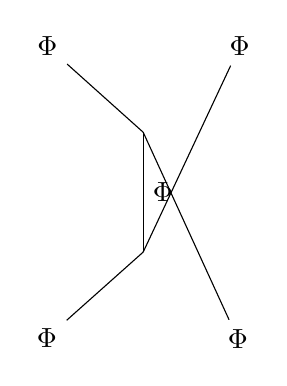
\begin{tikzpicture} % u-channel
\begin{feynman}
\diagram[vertical=x to y] {
    a [particle=\(\Phi\)] -- [plain] x -- [draw=none] c [particle=\(\Phi\)],
    b [particle=\(\Phi\)] -- [plain] y -- [draw=none] d [particle=\(\Phi\)],
    x -- [plain, edge label=\(\Phi\)] y
};
\diagram* {
    (x) -- [plain] (d) [particle=\(\Phi\)],
    (y) -- [plain] (c) [particle=\(\Phi\)]
};
\end{feynman}
\end{tikzpicture}
\]
By the same logic as before, there are 72 ways to get each of these diagrams. This means that, using these diagrams, we have accounted for $72*3 = 216$ fully contracted sets of field operators, which is exactly how many we had left unaccounted for earlier! Therefore, these three diagrams are the only diagrams which contribute. Therefore, summing everything together, the S-matrix is:
\[
S = \wick{\c1 \Phi_1 \c2 \Phi_2 \c1 \Phi_3 \c2 \Phi_4} + 
\wick{\c1 \Phi_1 \c2 \Phi_2 \c2 \Phi_3 \c1 \Phi_4} + 
\wick{\c1 \Phi_1 \c1 \Phi_2 \c2 \Phi_3 \c2 \Phi_4} + \]\[
72 \int \int d^4x d^4y (ig)^2 \wick{\c1 \Phi_1 \c2 \Phi_2 \c3 \Phi_3 \c4 \Phi_4 \c1 \Phi_x \c2 \Phi_x \c5 \Phi_x \c5 \Phi_y \c3 \Phi_y \c4 \Phi_y} + \]\[
72 \int \int d^4x d^4y (ig)^2 \wick{\c1 \Phi_1 \c2 \Phi_2 \c3 \Phi_3 \c4 \Phi_4 \c1 \Phi_x \c3 \Phi_x \c5 \Phi_x \c5 \Phi_y \c2 \Phi_y \c4 \Phi_y} + \]\[
72 \int \int d^4x d^4y (ig)^2 \wick{\c1 \Phi_1 \c2 \Phi_2 \c3 \Phi_3 \c4 \Phi_4 \c1 \Phi_x \c4 \Phi_x \c5 \Phi_x \c5 \Phi_y \c2 \Phi_y \c3 \Phi_y}
\]
Or, pictographically:

\[
S \approx 
\begin{tikzpicture}[scale=0.25]
\begin{feynman}
\diagram[horizontal=x to y] {
    a -- [draw=none] x -- [draw=none] b,
    c -- [draw=none] y -- [draw=none] d,
    x -- [draw=none] y,
    a -- [plain] c,
    b -- [plain] d
};
\end{feynman}
\end{tikzpicture} + 
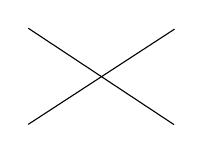
\begin{tikzpicture}[scale=0.5]
\begin{feynman}
\diagram[horizontal=x to y] {
    a -- [draw=none] x -- [draw=none] b,
    c -- [draw=none] y -- [draw=none] d,
    x -- [draw=none] y
};
\diagram* {
    (a) -- [plain] (d),
    (b) -- [plain] (c)
};
\end{feynman}
\end{tikzpicture} + 
\begin{tikzpicture}[scale=0.25]
\begin{feynman}
\diagram[horizontal=x to y] {
    a -- [draw=none] x -- [draw=none] b,
    c -- [draw=none] y -- [draw=none] d,
    x -- [draw=none] y,
    a -- [plain] b,
    c -- [plain] d
};
\end{feynman}
\end{tikzpicture} + 72
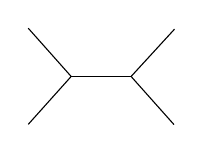
\begin{tikzpicture}[scale=0.5]
\begin{feynman}
\diagram[horizontal=x to y] {
    a -- x -- b,
    c -- y -- d,
    x -- y
};
\end{feynman}
\end{tikzpicture} + 72
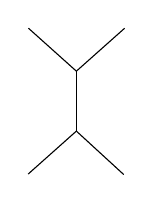
\begin{tikzpicture}[scale=0.5]
\begin{feynman}
\diagram[vertical=x to y] {
    a -- x -- b,
    c -- y -- d,
    x -- y
};
\end{feynman}
\end{tikzpicture} + 72
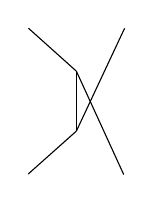
\begin{tikzpicture}[scale=0.5]
\begin{feynman}
\diagram[vertical=x to y] {
    a -- [plain] x -- [draw=none] c,
    b -- [plain] y -- [draw=none] d,
    x -- [plain] y
};
\diagram* {
    (x) -- [plain] (d),
    (y) -- [plain] (c)
};
\end{feynman}
\end{tikzpicture}
\]

Which is as far as we can go before working out how to evaluate these diagrams.

\section{$\Phi^4$}
The Procedure for $\Phi^4$ theory is very similar to that of $\Phi^3$ theory. The Lagrangian is $\mathcal{L} = \frac{1}{2}\partial_\mu \Phi \partial^\mu \Phi - \frac{1}{2}m^2\Phi^2 - \frac{g}{4!}\Phi^3$. Putting this into our Feynman path integral will yield all of the relevant diagrams for $\Phi\Phi \rightarrow \Phi\Phi$ scattering:
\[
\int \mathcal{D}[\Phi_1\Phi_2\Phi_3\Phi_4] e^{iS_0} \Phi_1\Phi_2\Phi_3\Phi_4 e^{i \int d^4x \mathcal{L}}
\]
Expanding the interaction term yields\footnote{Expansion here is done only to tree-order. The higher-order corrections will be addressed in a later section.}:
\[
\int \mathcal{D}[\Phi_1\Phi_2\Phi_3\Phi_4] e^{iS_0} \Phi_1\Phi_2\Phi_3\Phi_4 [1 - \frac{ig}{4!} \int d^4x \Phi^4(x)]
\]
This gives two terms. The first is the $\Phi\Phi \rightarrow \Phi\Phi$ free term, which we already know the diagrams for. The second term, however, is far more interesting. The field operators to be contracted are $\Phi_1\Phi_2\Phi_3\Phi_4\Phi_x\Phi_x\Phi_x\Phi_x$. The only connected diagram, then, is that in which all field operators corresponding to external states are contracted with one of the $\Phi_x$. There are $4!$ contractions that will cause this, giving a diagram:
\[
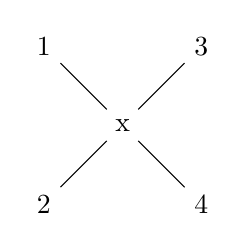
\begin{tikzpicture}
\begin{feynman}
    \vertex (a) at (-1, 1){1};
    \vertex (b) at (-1, -1){2};
    \vertex (c) at (1, 1){3};
    \vertex (d) at (1, -1){4};
    \vertex (x) at (0, 0){x};
\diagram*[horizontal=(a) to (x)] {
    (a) -- [plain] (x) -- [plain] (b),
    (c) -- [plain] (x) -- [plain] (d)
};
\end{feynman}
\end{tikzpicture}
\]
for the tree-level approximation of the $\Phi^4$ interaction. However, as with the $\Phi^3$ case, we cannot progress without knowing how to evaluate this diagram.

\chapter{Deriving the Feynman Rules}
It is all well and good that we can find the Feynman diagrams for these scattering processes, but let us not forget what we are truly interested in: the scattering matrix. Recall that the Feynman diagrams are simply placeholders for more complex mathematical expressions. The process for computing the scattering matrix is therefore one of decoding the Feynman diagrams into their mathematical expressions, then evaluating them.

Thankfully, the way that Feynman diagrams are evaluated is relatively straightforward. Feynman diagrams consist of many components (lines and vertices), which are each associated with a mathematical term. The term for the entire diagram is the product of each of its constituent terms. A process with multiply diagrams is represented by the sum of the terms for each of its diagrams.

Logically, there are three parts to a Feynman diagram: external lines, vertices, and internal lines. Each of these parts, as mentioned before, has some associated term. Each part can be considered in turn. In scalar field theory, external lines contribute a factor of $1$, making them essentially irrelevant to the calculation altogether. Unfortunately, this is not the case for particles with spin.

The vertex factors we have already inadvertently dealt with. When Taylor expanding out the interaction term in the path integral, the nth term picked up the coefficient of $i$ times the Lagrangian's interaction term's coefficient, all to the nth power. For instance, in $\Phi^3$ theory, the terms had coefficients $1$, $\frac{ig}{3!}$, $(\frac{ig}{3!})^2$, and so on. Likewise, in $\Phi^4$ theory, the terms had coefficients $1$, $\frac{ig}{4!}$, $\frac{ig}{4!}$, etc. This corresponds to the interaction Lagrangian coefficients of $\frac{g}{3!}$ and $\frac{g}{4!}$, respectively. The nth term in the expansion governs all diagrams with n vertices. It stands to reason from these two observations that each vertex contributes a factor of $i$ times the interaction Lagrangian's coefficient. As it turns out, this relationship holds not only in scalar field theory, but in all quantum field theories.

Lastly, the internal lines contribute factors called propagators, as they represent the propagation of a particle from one point to another. Calculating propagators is a quite involved process, beginning with the realization that propagators are Green's functions of equations of motion (times $i$). Therefore, the process is two-stepped: first find the equation of motion of the particle, then find the Green's function of that equation of motion. The remained of this section will consist of said derivation, which can be skipped by those lacking either the mathematical background or willpower to follow along.

For the scalar particle, no matter the scattering process or interaction considered, the free Lagrangian is $\mathcal{L} = \frac{1}{2}\partial_\mu \Phi \partial^\mu \Phi - \frac{1}{2}m^2 \Phi^2$. The rules of Lagrangian mechanics tell us that the equation of motion of the particle will be the Euler-Lagrange equation that follows from this Lagrangian. The Euler-Lagrange equation is $\frac{\partial \mathcal{L}}{\partial \Phi} = \partial_\mu \frac{\partial \mathcal{L}}{\partial (\partial_\mu \Phi)}$. Therefore, the equation of motion of a free, scalar particle is:
\[
\frac{\partial}{\partial \Phi} (\frac{1}{2}\partial_\mu \Phi \partial^\mu \Phi - \frac{1}{2}m^2 \Phi^2) = \partial_\mu \frac{\partial}{\partial (\partial_\mu \Phi)} (\frac{1}{2}\partial_\mu \Phi \partial^\mu \Phi - \frac{1}{2}m^2 \Phi^2)
\]
\[
-m^2 \Phi = \partial_\mu \frac{\partial}{\partial (\partial_\mu \Phi)} (\frac{1}{2}g^{\mu\nu}(\partial_\mu \Phi)^2)
\]
\[
-m^2 \Phi = \partial_\mu g^{\mu\nu} \partial_\mu \Phi
\]
\[
-m^2 \Phi = \partial_\mu \partial^\mu \Phi
\]
\[
(\Box^2 + m^2) \Phi = 0
\]
This final equation is very famous and is known as the Klein-Gordon equation. It is the equation of motion of a free, scalar particle. The next step, as mentioned before, is to find the Green's function of this equation.

The Green's function of an operator $\hat{L}$ is the function $G(x)$ such that $\hat{L}G(x) = \delta(x)$. The operator for the Klein-Gordon equation is $\Box^2 + m^2$, meaning the Green's function must satisfy $(\Box^2 + m^2) G(x) = \delta(x)$. It is beyond the scope of this discussion to prove that the solution is:
\[
G(x) = \int \frac{d^4}{(2\pi)^4} \frac{1}{p^2 - m^2} e^{i \vec{x} \cdot \vec{p}}
\]
where $\vec{x}$ and $\vec{p}$ are the corresponding 3-vectors to $x^\mu$ and $p^\mu$. This expression seems to be heavily suggesting a Fourier transform, as the 4-D inverse Fourier transform of a function $\Tilde{f}(p)$ in momentum space is $\int \frac{d^4}{(2\pi)^4} \Tilde{f}(p) e^{i \vec{x} \dot \vec{p}}$. Therefore, the convention is (sensibly) to switch to momentum space when analyzing Feynman diagrams, only converting to position space when absolutely necessary. In momentum space, the scalar propagator is simply $\frac{i}{p^2 - m^2}$. It is worth noting that this shift to momentum space will not affect the vertex term nor external term.

There is a fundamental law of nature which has not yet been taken into account: conservation of momentum. At each vertex, momentum should be conserved. This can be accomplished by integrating over all internal momenta and adding a delta function for each vertex.

To make the connection between these expressions and their Feynman diagrams clearer, the contribution for each part of the diagram is often used as a label for the part which contributed it. For instance, the s-channel diagram
\[
\begin{tikzpicture}
\begin{feynman}
\diagram[horizontal=x to y]{
    a -- [plain] x -- [plain] b,
    c -- [plain] y -- [plain] d,
    x -- [plain, momentum=$p$] y
};
\end{feynman}
\end{tikzpicture}
\]
can be drawn

\[
\feynmandiagram[horizontal=x to y]{
    a [particle=\(\Phi_2\)] -- [plain] x [label=180:$ig$] -- [plain] b [particle=\(\Phi_1\)],
    c [particle=\(\Phi_4\)] -- [plain] y [label=0:$ig$] -- [plain] d [particle=\(\Phi_3\)],
    x -- [plain, edge label=$\frac{i}{p^2 - m^2}$] y
};
\]

making it much clearer that the overall diagram yields the term $(ig)^2 \int \frac{d^4p}{(2\pi)^2} \frac{i}{p^2 - m^2} \delta(p_1 + p_2 - p) \delta(p - p_3 - p_4)$.

What we are interested in is the matrix element of the scattering matrix, often denoted $\mathcal{M}$. Strictly speaking, the evaluation of a Feynman diagram is equal to $i\mathcal{M}\delta(p_{in} - p_{out})$. Therefore, the s-channel diagram has\footnote{The tilde over the $\mathcal{M}$ denotes that this is the momentum-space matrix element.}:
\[
i \Tilde{\mathcal{M}} \delta(p_{in} - p_{out}) = (ig)^2 \int \frac{d^4p}{(2\pi)^2} \frac{i}{p^2 - m^2} \delta(p_1 + p_2 - p) \delta(p - p_3 - p_4)
\]
But, using the identity $\int f(x) \delta(x - a) dx = f(a)$:
\[
i \Tilde{\mathcal{M}} \delta(p_{in} - p_{out}) = (ig)^2 \frac{1}{(2\pi)^2} \frac{i}{(p_1 + p_2)^2 - m^2} \delta(p_1 + p_2 - p_3 - p_4)
\]
So:
\[
\Tilde{\mathcal{M}} = (ig)^2 \frac{1}{(2\pi)^4} \frac{1}{(p_1 + p_2)^2 - m^2}
\]
This is the first of many scattering matrix elements we will evaluate in quantum field theory. Though the math was very intensive, this model is far more accurate and more useful than that of non-relativistic quantum mechanics. Also note that the integral nicely cancelled due to the delta function. This does not always occur, but it is very nice when it does.

\section{Off-Shell Particles}
Very astute readers will notice at this point that we have seemingly divided by 0 in the propagator. General relativity tells us that, for a massive particle, $p^2 = m^2$. Therefore, the propagator $\frac{i}{p^2 - m^2}$ is problematic. However, quantum field theory has been used to predict values which have later been experimentally verified. How can this be possible? The answer is virtual particles.

The internal lines in a Feynman diagram represent virtual particles. They cannot be directly observed, and they necessarily have exceedingly short lifetimes. The rules of quantum mechanics tell us that some laws of physics can be seemingly violated so long as the duration is short enough to bring the Heisenberg uncertainty principle into play. These virtual particles simply do not follow the rule $p^2 = m^2$. This is known as being "off-shell". As it turns out, all that is necessary as far as momentum goes is that 4-momentum be conserved at each vertex and that real particles be on-shell.

\section{Mandelstam Variables}
Before we go about calculating matrix elements, there is a useful notational trick that will make the calculations slightly easier. In tree-level diagrams, we oftentimes deal with the square of the magnitude of an internal propagator's momentum. For instance, in the t-channel diagram we dealt with before, there was a factor of $\frac{i}{p^2 - m^2}$. We introduce a new variable, $t$, equal to $p^2$. Therefore, the propagator is $\frac{i}{t - m^2}$. While this may seem like a slight difference, it ends up making many calculations more compact and easier to deal with.

Likewise, we can apply the same logic to the s-channel and u-channel diagrams, defining $s$ and $u$ as $p^2$, respectively. This means that the following identities are true:
\[
s = (p_1 + p_2)^2 = (p_3 + p_4)^2 = E_{CM}^2
\]
\[
t = (p_1 - p_3)^2 = (p_2 - p_4)^2
\]
\[
u = (p_1 - p_4)^2 = (p_2 - p_3)^2
\]
These variables are known as Mandelstam variables.

\chapter{Tree Level Matrix Elements in Scalar Field Theory}
\section{Matrix Element Norm Squared}
As quantum mechanics reveals, while most quantities can be complex numbers, it is the norm squared of the quantity which is a real observable. This is true for the matrix element in quantum field theory. Therefore, while the matrix element itself is derived from Feynman diagrams, only the matrix element's norm squared will be truly measurable. This comes into play far more in theories more complex than scalar field theory, where the norm squared of the matrix element will, in fact, be of a simpler form than the matrix element itself.

\section{$\Phi^4$}
Finally, we are ready to calculate an S-matrix element. As evaluated before from the Feynman path integral expansion, the only tree-level, connected diagram is, with multiplicity $4!$:
\[
\feynmandiagram[horizontal=x to y]{
    a [particle=\($\Phi$\)] -- [plain] x -- [plain] b [particle=\($\Phi$\)],
    c [particle=\($\Phi$\)] -- [plain] x -- [plain] d [particle=\($\Phi$\)]
};
\]
Therefore, applying the Feynman rules for scalar field theory:
\[
i \mathcal{M} \delta (p_{in} - p_{out}) = 4! \frac{ig}{4!} \delta (p_1 + p_2 - p_3 - p_4)
\]
So, quite simply:
\[
\mathcal{M} = g
\]
This is a remarkably concise matrix element. Unfortunately, other matrix elements will hardly be so kind. However, it is the norm squared of the matrix element which has physical meaning. Therefore, our final result is simply:
\[
\vert \mathcal{M} \vert ^2 = g^2
\]

\section{$\Phi^3$}
The scattering matrix element of $\Phi^3$ is, unfortunately, significantly more complicated. The tree-level Feynman diagrams are the t, s, and u-channel diagrams with which we have become familiar:
% All of the diagrams with proper labelling
where we have redefined $g$ to include the factors of $frac{1}{3!}$. We can now apply the Feynman rules to find:
\[
i \mathcal{M}_s \delta (\Delta p) = 
(ig)^2 \int \frac{d^4p}{(2\pi)^4}
\frac{i}{p^2 - m^2}
\delta(p_1 + p_2 - p) \delta(p - p_3 - p_4)
\]
\[
i \mathcal{M}_t \delta (\Delta p) = 
(ig)^2 \int \frac{d^4p}{(2\pi)^4}
\frac{i}{p^2 - m^2}
\delta(p_1 - p - p_3) \delta(p_2 + p - p_4)
\]
\[
i \mathcal{M}_u \delta (\Delta p) = 
(ig)^2 \int \frac{d^4p}{(2\pi)^4}
\frac{i}{p^2 - m^2}
\delta(p_1 - p - p_4) \delta(p_2 + p - p_3)
\]

So, applying the delta functions and simplifying:
\[
\mathcal{M}_s = (ig)^2 \frac{1}{s - m^2}
\]
\[
\mathcal{M}_t = (ig)^2 \frac{1}{t - m^2}
\]
\[
\mathcal{M}_u = (ig)^2 \frac{1}{u - m^2}
\]
Now that we have all of the matrix elements, we can add them to find the overall matrix element:
\[
\mathcal{M} = \mathcal{M}_s + \mathcal{M}_t + \mathcal{M}_u = 
(ig)^2 (\frac{1}{s - m^2} + \frac{1}{t - m^2} + \frac{1}{u - m^2})
\]
Again, through, it is the norm squared of the matrix element which matters for physical predictions:
\[
\vert \mathcal{M} \vert ^2 = g^4 (\frac{1}{s - m^2} + \frac{1}{t - m^2} + \frac{1}{u - m^2})^2
\]

\subsection{Boundary Cases}
There are two important boundary cases to examine for any result in quantum field theory: the low-energy limit and the high-energy, or relativistic limit. The former assumes that nothing is moving with particularly high energy nor momentum, and therefore $s$, $t$, and $u$ approach 0. In this limit, the norm-squared of the S-matrix element approaches:
\[
\lim_{s,t,u \rightarrow 0} \vert \mathcal{M} \vert ^2 = \frac{9g^4}{m^4}.
\]
That is, when all particles involved are moving relatively slowly, the s-matrix element is greater when the interaction is stronger and the particles involved are lighter.

As it turns out, the relativistic limit is slightly more involved. In that limit, the incoming energies are very high, and the differences in energies are therefore also higher, meaning that $s$, $t$, and $u$ are all much greater than $m^2$. The norm-squared of the S-matrix element in this limit approaches:
\[
\lim_{s,t,u \gg m^2} \vert \mathcal{M} \vert ^2 =
g^4 (\frac{1}{s} + \frac{1}{t} + \frac{1}{u})
\]
As the momenta continue to increase, the overall matrix element will tend to 0, reflecting the fact that it is harder to generate collisions between particles moving at relativistic speeds than ones moving at more manageable speeds. Interactions occur with less frequency simply because the particles are less likely to scatter off of one another in the first place.

\chapter{Loops and Renormalization}
A keen-eyed reader may have noticed by this point that all diagrams considered thus far have been low-enough order to be lacking something which appears in nearly all higher-order diagrams: loops. As it turns out, loops are the bane of the existences of quantum field theorists, as they present a unique mathematical challenge. The issues lies in the fact that while observable quantities must be finite, terms in the intermediate steps of a calculation need not be so kind. Therefore, it is possible for infinities to appear in calculations which should yield finite answers, thereby requiring some mathematical trickery in order to massage the expression in such a way as to handle the infinity until it is properly removed from the expression. This is exactly the issue presented by loops in Feynman diagrams, and the process of removing these infinities is known as renormalization. Unfortunately, this chapter is very mathematically dense, and therefore may be best skipped by those simply dipping their toes into the physics.

\section{$g^2$ Term in $\Phi^4$}
The next-order contribution in $\Phi^4$ theory includes the $g^2$ order diagram:
% Insert diagram (s-channel)
\[
\feynmandiagram[horizontal=x to y]{
    a -- [plain] x [label=180:$ig$] -- [plain] b,
    c -- [plain] y [label=0:$ig$] -- [plain] d,
    x -- [half left, momentum=\(k\)] y,
    y -- [half left, momentum=\(q\)] x
};
\]

From the Feynman rules, we know that it contributes a term:
\[
i \mathcal{M} \delta (\Delta p) = (ig)^2 \int \frac{d^4q}{(2\pi)^4} \int \frac{d^4k}{(2\pi)^4} \frac{i}{k^2 - m^2} \frac{i}{q^2 - m^2} \delta(p_1 + p_2 - k - q) \delta(k + q - p_3 - p_4)
\]
So:
\[
i \mathcal{M} = (ig)^2 \int \frac{d^4k}{(2\pi)^4} \frac{i}{k^2 - m^2} \frac{i}{(p - k)^2 - m^2}
\]
Notice that, unlike before, an integral remains which is not cancelled by a delta function. This presents quite the problem, as the integral diverges. However, we know that the final result does not diverge, and so there must be some trick in order to yield a finite result despite an infinite intermediary. As it turns out, the solution has two steps: the use the Feynman parameter followed by the use of the Pauli-Villars regulator. These two steps will together renormalize this integral into something finite.

\subsection{The Feynman Parameter}
The integral we are dealing with is, to be specific, logarithmically divergent. This is because the power of the integral is the inverse of the power of the integrand. That is, we have an integrand proportional to $\frac{1}{k^4}$, and we are integrating with respect to $d^4 k$. This means that the final result ought to have the form of a logarithm. We will see in time that this is the case. For now, a number of steps will be taken in order to massage the integral into a nicer form so that the Pauli-Villars regularization scheme may be undergone.

First, notice the following trivial identity which appears needlessly over-complicated:
\[
\frac{1}{AB} = \int_0^1 dx \frac{1}{[A + (A - B)x]^2}
\]
We can apply this to the integrand of our desired integral, letting $A = k^2 - m^2$ and $B = (p - k)^2 - m^2$:
\[
\frac{1}{k^2 - m^2} \frac{1}{(p - k)^2 - m^2} = \int_0^1 dx \frac{1}{[k^2 - m^2 + (k^2 - m^2 - (p - k)^2 + m^2)x]^2}
\]
\[
= \int_0^1 dx \frac{1}{[k^2 - m^2 + (k^2 - (p - k)^2)x]^2} = \int_0^1 dx \frac{1}{[k^2 - m^2 + k^2x - (p - k)^2x]^2}
\]
\[
\int_0^1 dx \frac{1}{[k^2 - m^2 + k^2x - p^2x - k^2x - 2pkx]^2} = \int_0^1 dx \frac{1}{[k^2 - m^2 - p^2x - 2pkx]^2}
\]
Now, in the denominator, we can complete the square, yielding:
\[
\int_0^1 dx \frac{1}{[(k - px)^2 - m^2 + p^2x - p^2x^2]^2}
\]
Without changing the integration measure, we can redefine $k \rightarrow k + px$. We can also define $\Delta^2 = m^2 - p^2x + p^2x^2$. This turns the integral into the much simpler form:
\[
\int_0^1 dx \frac{1}{[k^2 - \Delta^2]^2}
\]
However, this was simply the integrand of the original integral. In all, we have:
\[
i \mathcal{M} = (ig)^2 \int \frac{d^4k}{(2\pi)^4} \frac{i}{k^2 - m^2} \frac{i}{(p - k)^2 - m^2} = -(ig)^2 \int_0^1 dx \int \frac{d^4k}{(2\pi)^4} \frac{1}{[k^2 - \Delta^2]^2}
\]

\subsection{The Pauli-Villars Regulator}
The Pauli-Villars regularization scheme involves adding a new term to the Lagrangian describing a new particle which only ever exists in diagram as a virtual particle, then at the end taking the limit as that particle's terms in the Lagrangian approach 0. The exact process of this will not be undergone, but the aspect important to our purposes is that a new diagram involving an interaction mediated by this particle will add its own contribution, giving us a new expression for the S-matrix element\footnote{After this point, the limit for the $\Lambda$ will be implicit.}:
\[
i \mathcal{M} = \lim_{\Lambda \rightarrow \infty} -(ig)^2 \int_0^1 dx \int \frac{d^4k}{(2\pi)^4} (\frac{1}{[k^2 - \Delta^2]^2} - \frac{1}{[k^2 - \Lambda^2]^2})
\]
Because the integrand depends only on the magnitude of $k$, this integral can be much easier evaluated in the 4-dimensional analog to spherical coordinates\footnote{Strictly speaking, a Wick rotation is needed in order to make this possible as a (++++) metric signature as opposed to a (+---) metric signature would be necessary. However, Wick rotations are outside the scope of this discussion, and so the effects of one will be ignored.}. This gives the integral:
\[
i \mathcal{M} = \lim_{\Lambda \rightarrow \infty} -(ig)^2 \int_0^1 dx \int d^3\Omega_3 \int_0^{\infty} \frac{dk}{(2\pi)^4} k^3 (\frac{1}{[k^2 - \Delta^2]^2} - \frac{1}{[k^2 - \Lambda^2]^2})
\]
\[
i \mathcal{M} = \lim_{\Lambda \rightarrow \infty} -(ig)^2 \frac{2\pi^2}{(2\pi)^4}  \int_0^1 dx \int_0^{\infty} dk (\frac{k^3}{[k^2 - \Delta^2]^2} - \frac{k^3}{[k^2 - \Lambda^2]^2})
\]
This integral is finally calculable, and it gives:
\[
i \mathcal{M} = \lim_{\Lambda \rightarrow \infty} -(ig)^2 \frac{1}{8\pi^2}  \int_0^1 ln(\frac{\Delta^2}{\Lambda^2}) dx
\]
Inserting the expression for $\Delta$ gives:
\[
i \mathcal{M} = \lim_{\Lambda \rightarrow \infty} -(ig)^2 \frac{1}{8\pi^2}  \int_0^1 ln(\frac{m^2 - p^2x + p^2x^2}{\Lambda^2}) dx
\]
Unfortunately, the integral with respect to the dummy variable $x$ is somewhat ugly, and therefore not worth writing out in full here. However, in the case of a specific scattering experiment, it could be evaluated with a calculator.

\section{Non-Renormalizability of Gravity}
There have been many attempts to apply the success of quantum field theory to gravity. However, it has never quite properly worked, for a variety of reasons. One such issue is that gravitation is a "non-renormalizable theory". That is, it cannot be renormalized in the way that the other, quantum, theories can. When renormalizing the higher-order term in $\Phi^4$ theory using the Pauli-Villars regulator, only one counter-term needed to be added to the Lagrangian in order to finitize the integral. In other theories, more counter-terms may be needed. However, gravity is non-renormalizable because it cannot be renormalized with a finite number of counter-terms. Instead, an infinite number of these additional terms would be needed in order to finitize the integral. Therefore, a different method is required. As it turns out, no regularization method quite does the trick for gravity. This is what has led to far more complex theories such as String Theory and M-Theory, which are designed to be able to wrangle these infinities which are produced when attempting to quantize gravity.

\chapter{The Quantum Field Theory Procedure}
Though it is the only theory we have dealt with (and, in fact, the only theory we will deal with), scalar field theory is but the simplest of many quantum field theories. Quantum electrodynamics, quantum chromodynamics, and electroweak theory are the shining examples of more complex, but more predictive theories for how the universe behaves. Though the mathematics governing these theories are more complicated than that governing scalar field theory, the procedure for analyzing scattering events is the same for any type of quantum field theory.

As we have learned from scalar field theory, the Lagrangian is the starting point for the description of a theory. First, the relevant Lagrangian for the desired theory must be ascertained. See Appendix A for the process by which the scalar field theory Lagrangian is derived. For other theories, similar lines of reasoning must be followed. The Lagrangian provides a very precise encapsulation of the way that things move in the theory both freely and during interactions.

The next step is to determine all of the Feynman diagrams associated with the theory. This is done by evaluating all of the possible contractions of the field operators in each order of the expansion of the Feynman path integral, a process first encountered in Chapter 5. Then, only the connected diagrams relevant to the specific scattering process being considered can be taken into account, with the extraneous diagrams being ignored.

At this point, the Feynman diagrams must be translated into precise mathematical statements according to the Feynman rules. Therefore, at this stage, the Feynman rules must be derived. There are three types of factors to be determined: propagators, vertex factors, and external factors. Propagators are found by working out the Green's function of the Euler-Lagrange equation generated by the theory's free Lagrangian, and multiplying it by $i$. That description contains quite a bit of jargon, but Chapter 7 walks through the derivation for scalar field theory nicely. Vertex factors are found from the coefficient of each term of the expansion of the path integral, which was done when the Feynman diagram were found in the previous step. Each vertex should give one additional vertex factor. Finally, the external vertices come from the spin states and polarization states of incoming and outgoing particles. Because scalars have no spin nor polarization, external factors are not considered here whatsoever.

If necessary, some terms may need to be renormalized. This can be done any of a large number of ways. Here, we have only covered dimensional regularization, but many others exist.

Now that each diagram can be converted into a precise mathematical expression via the Feynman rules, all that remains is to combine and simplify the expressions. S-matrix elements for each diagram should be added together in order to find the matrix element for the process altogether. Then, the norm squared of the S-matrix element should be found. This leaves only the task of simplifying the expression and considering any relevant boundary cases.

In more condensed form, the quantum field theory procedure is:
\begin{enumerate}
    \item Determine the Lagrangian of the theory
    \item Find all of the relevant Feynman diagrams
    \item Determine the Feynman rules
    \begin{itemize}
        \item Find the propagators from the Green's function of the free Lagrangian's Euler-Lagrange equation
        \item Find the vertex factors from the interaction term of the Lagrangian, or the expansion of the path integral
        \item Find the external factors from the spin states and polarization states
    \end{itemize}
    
    \item Find the expression for each Feynman diagram
    \item Renormalize, if necessary
    \item Find the norm squared of the matrix element and simplify
\end{enumerate}

\begin{appendices}
\chapter{Lagrangians}
The Lagrangian of a system is the kinetic energy minus the potential energy. It is the key object of study in Lagrangian mechanics, as it has the very important property that the path taken by an object is always the one which minimizes or maximises the time-integral of the Lagrangian\footnote{This quantity is known as the action, hence the commonly known, "Principle of Least Action" or, more aptly, "Principle of Stationary Action".}. In quantum field theory, we will technically deal with the Lagrangian density, though it will be referred to simply as the Lagrangian for brevity.

As it turns out, there will be three types of terms to consider in the Lagrangian for a quantum field theory: kinetic terms, mass terms, and interaction terms. Kinetic terms are straightforward: they correspond to the energy the excitations of the field have due to their motion. The mass term represents the energy it takes to set up the field in the first place. It is akin to the rest energy of the field configuration. Finally, interaction terms are the terms corresponding to the potential energy stored in interactions between particles.

It is worth noting that there are many Lagrangians that could equally describe scalar field theory. However, the one most commonly used ($\mathcal{L} = \frac{1}{2}\partial_\mu\Phi\partial^\mu\Phi - \frac{1}{2}m^2\Phi^2$) is the simplest. Thankfully, it is relatively easy to derive.

To begin, it is vital to note that the Lagrangian is a function of only the field configuration $\Phi$ and its first derivative $\partial_\mu\Phi$, as well as that it is a Lorentz scalar, meaning that it is the same for all observers. The first point is simply an assertion, while the latter comes from the reasoning while many properties of objects are relative, their equations of motion are not. Therefore, their Lagrangians must too be relativistically invariant, which is equivalent to being a Lorentz scalar.

Terms without derivatives roughly correspond to interactions. For instance, a Lagrangian term of $\lambda ABC$ would correspond to the vertex connecting a propagator for an $A$ particle, a $B$ particle, and a $C$ particle. $\lambda$ is the coupling constant, which relates to the interaction strength. Therefore, the free Lagrangian cannot contain any terms without derivatives of an order higher than $\Phi^2$, as it would correspond to a vertex containing more than a simple in and out of a particle, which would be, by definition, an interaction.

The simplest imaginable Lagrangian which follows these tenets is:
\[
\mathcal{L} = a \partial_\mu\Phi\partial^\mu\Phi - b \Phi - c \Phi^2
\]
One may be wondering why there are no terms containing both $\Phi$ and its derivative. The simple reason is that such terms are, indeed, possible. In fact, there are used in some types of renormalization, such as Pauli-Villars Regulatization. However, it turns out that they are simply not needed, and therefore are to be left out of our "simplest possible Lagrangian".

Additionally, one may be confused as to why the derivative has to appear in the way that it does (contracted with itself). The answer is simply that there is no other way to make the term be a scalar overall than to contract the derivative with itself, as the only way to produce a Lorentz scalar from a vector or a dual vector is through a contraction, and there is no other vector (or dual vector) with which to contract.

One useful property of the Lagrangian is that is it positive-definite. The concept of positive-definiteness is beyond the scope of this discussion, but it is sufficient to explain that the term linear in $\Phi$ ruins any hope of this Lagrangian being positive-definite. Therefore, we set $b$ to 0, bringing us very close to the desired Lagrangian.

In order to keep the units the same across all terms, the term quadratic in $\Phi$ must contain a coefficient proportional to $m^2$. As a convention, the entire Lagrangian density picks up a factor of $\frac{1}{2}$, simply to make some of the math easier. Therefore, we have arrived exactly at the desired Lagrangian for scalar field theory:
\[
\mathcal{L} = \frac{1}{2}\partial_\mu\Phi\partial^\mu\Phi - \frac{1}{2}m^2\Phi^2
\]
Where interaction terms can be added as needed in order to analyze different types of interactions, such as $g \Phi^3$ or $g \Phi^4$.

\chapter{Fourier Transforms}
As it turns out, some quantities have an intrinsic relationship with one other, known as being Fourier conjugates. The simplest example of this is time and frequency. For each (integrable) function of some variable, there exists another function, the Fourier transform of the first function, which is a function of the Fourier conjugate of the variable. A very common example of this is the decomposition of sound waves via Fourier analysis. A function of time which is a sum of many sinusoidal functions with different frequencies can be Fourier transformed into a function of frequency, which would have peaks at the points of the frequencies composing the original sinusoidal function, with the height of the peak corresponding to the coefficient of the sine function producing that frequency.

The formula for the Fourier transform of a function is relatively straightforward. For a function $f(t)$, the Fourier transform is:
\[
\Tilde{f}(\tau) = \frac{1}{2\pi} \int_{-\infty}^{\infty} f(t)e^{-t\tau} dt
\]
where $\tau$ is the Fourier conjugate variable to $t$.

As it turns out, variables which are Fourier conjugates will have quantum operators which do not commute. This reveals the deep connection between Fourier analysis and quantum mechanics, as position and momentum are Fourier conjugates. This means that any function of position $f(x)$ has a corresponding function of momentum $k$:
\[
\pi(k) = \frac{1}{2\pi} \int_{-\infty}^{\infty} f(x)e^{-kx} dx
\]
which can be reversed via the inverse Fourier transform:
\[
f(x) = \frac{1}{2\pi} \int_{-\infty}^{\infty} \pi(k) e^{kx} dk
\]
The wavefunction itself, for instance, has a Fourier transform "momentum-space wavefunction" which behaves with respect to momentum in exactly the same way as the position-space wavefunction does with respect to position, and vice-versa.

The Fourier transform can be easily extended to higher dimensions, as well. A position-space function and a momentum-space function in $D$ dimensions relate to one another by:
\[
\pi(k) = \int_{-\infty}^{\infty} \frac{d^D x}{(2\pi)^D} f(x)e^{-k \cdot x}
\]
\[
f(x) = \int_{-\infty}^{\infty} \frac{d^D x}{(2\pi)^D} \pi(k) e^{k \cdot x}
\]

\end{appendices}
\end{document}
